
%% bare_jrnl.tex
%% V1.3
%% 2007/01/11
%% by Michael Shell
%% see http://www.michaelshell.org/
%% for current contact information.
%%
%% This is a skeleton file demonstrating the use of IEEEtran.cls
%% (requires IEEEtran.cls version 1.7 or later) with an IEEE journal paper.
%%
%% Support sites:
%% http://www.michaelshell.org/tex/ieeetran/
%% http://www.ctan.org/tex-archive/macros/latex/contrib/IEEEtran/
%% and
%% http://www.ieee.org/



% *** Authors should verify (and, if needed, correct) their LaTeX system  ***
% *** with the testflow diagnostic prior to trusting their LaTeX platform ***
% *** with production work. IEEE's font choices can trigger bugs that do  ***
% *** not appear when using other class files.                            ***
% The testflow support page is at:
% http://www.michaelshell.org/tex/testflow/


%%*************************************************************************
%% Legal Notice:
%% This code is offered as-is without any warranty either expressed or
%% implied; without even the implied warranty of MERCHANTABILITY or
%% FITNESS FOR A PARTICULAR PURPOSE! 
%% User assumes all risk.
%% In no event shall IEEE or any contributor to this code be liable for
%% any damages or losses, including, but not limited to, incidental,
%% consequential, or any other damages, resulting from the use or misuse
%% of any information contained here.
%%
%% All comments are the opinions of their respective authors and are not
%% necessarily endorsed by the IEEE.
%%
%% This work is distributed under the LaTeX Project Public License (LPPL)
%% ( http://www.latex-project.org/ ) version 1.3, and may be freely used,
%% distributed and modified. A copy of the LPPL, version 1.3, is included
%% in the base LaTeX documentation of all distributions of LaTeX released
%% 2003/12/01 or later.
%% Retain all contribution notices and credits.
%% ** Modified files should be clearly indicated as such, including  **
%% ** renaming them and changing author support contact information. **
%%
%% File list of work: IEEEtran.cls, IEEEtran_HOWTO.pdf, bare_adv.tex,
%%                    bare_conf.tex, bare_jrnl.tex, bare_jrnl_compsoc.tex
%%*************************************************************************

% Note that the a4paper option is mainly intended so that authors in
% countries using A4 can easily print to A4 and see how their papers will
% look in print - the typesetting of the document will not typically be
% affected with changes in paper size (but the bottom and side margins will).
% Use the testflow package mentioned above to verify correct handling of
% both paper sizes by the user's LaTeX system.
%
% Also note that the "draftcls" or "draftclsnofoot", not "draft", option
% should be used if it is desired that the figures are to be displayed in
% draft mode.
%

\documentclass[technote]{IEEEtran}
%\documentclass[draftcls]{IEEEtran}


%\usepackage{graphicx}
\usepackage{type1cm}
\usepackage{eso-pic}
\usepackage{color}

\makeatletter
\AddToShipoutPicture{%
            \setlength{\@tempdimb}{.5\paperwidth}%
            \setlength{\@tempdimc}{.5\paperheight}%
            \setlength{\unitlength}{1pt}%
            \put(\strip@pt\@tempdimb,\strip@pt\@tempdimc){%
        \makebox(0,0){\rotatebox{45}{\textcolor[gray]{0.95}%
        {\fontsize{6cm}{6cm}\selectfont{DRAFT}}}}%
            }%
}
\makeatother

% If IEEEtran.cls has not been installed into the LaTeX system files,
% manually specify the path to it like:
% \documentclass[journal]{../sty/IEEEtran}
\makeatletter
\def\markboth#1#2{\def\leftmark{\@IEEEcompsoconly{\sffamily}
\MakeUppercase{\protect#1}}%
\def\rightmark{\@IEEEcompsoconly{\sffamily}
\MakeUppercase{\protect#2}}}
\makeatother

\usepackage[italian]{babel}
\usepackage[utf8]{inputenc}

%\renewcommand{\vec}[1]{\mathbf{#1}}
\newcommand{\mat}[1]{\mathbf{#1}}
\usepackage{color}
\newcommand{\hilight}[1]{\colorbox{yellow}{#1}}


% Some very useful LaTeX packages include:
% (uncomment the ones you want to load)


% *** MISC UTILITY PACKAGES ***
%
%\usepackage{ifpdf}
% Heiko Oberdiek's ifpdf.sty is very useful if you need conditional
% compilation based on whether the output is pdf or dvi.
% usage:
% \ifpdf
%   % pdf code
% \else
%   % dvi code
% \fi
% The latest version of ifpdf.sty can be obtained from:
% http://www.ctan.org/tex-archive/macros/latex/contrib/oberdiek/
% Also, note that IEEEtran.cls V1.7 and later provides a builtin
% \ifCLASSINFOpdf conditional that works the same way.
% When switching from latex to pdflatex and vice-versa, the compiler may
% have to be run twice to clear warning/error messages.






% *** CITATION PACKAGES ***
%
%\usepackage{cite}
% cite.sty was written by Donald Arseneau
% V1.6 and later of IEEEtran pre-defines the format of the cite.sty package
% \cite{} output to follow that of IEEE. Loading the cite package will
% result in citation numbers being automatically sorted and properly
% "compressed/ranged". e.g., [1], [9], [2], [7], [5], [6] without using
% cite.sty will become [1], [2], [5]--[7], [9] using cite.sty. cite.sty's
% \cite will automatically add leading space, if needed. Use cite.sty's
% noadjust option (cite.sty V3.8 and later) if you want to turn this off.
% cite.sty is already installed on most LaTeX systems. Be sure and use
% version 4.0 (2003-05-27) and later if using hyperref.sty. cite.sty does
% not currently provide for hyperlinked citations.
% The latest version can be obtained at:
% http://www.ctan.org/tex-archive/macros/latex/contrib/cite/
% The documentation is contained in the cite.sty file itself.






% *** GRAPHICS RELATED PACKAGES ***
%
\ifCLASSINFOpdf
  % \usepackage[pdftex]{graphicx}
  % declare the path(s) where your graphic files are
  % \graphicspath{{../pdf/}{../jpeg/}}
  % and their extensions so you won't have to specify these with
  % every instance of \includegraphics
  % \DeclareGraphicsExtensions{.pdf,.jpeg,.png}
  \usepackage[pdftex]{graphicx}
  \graphicspath{{img}}
  \DeclareGraphicsExtensions{.pdf,.jpeg,.png}
\else
  % or other class option (dvipsone, dvipdf, if not using dvips). graphicx
  % will default to the driver specified in the system graphics.cfg if no
  % driver is specified.
  % \usepackage[dvips]{graphicx}
  % declare the path(s) where your graphic files are
  % \graphicspath{{../eps/}}
  % and their extensions so you won't have to specify these with
  % every instance of \includegraphics
  % \DeclareGraphicsExtensions{.eps}
\fi
% graphicx was written by David Carlisle and Sebastian Rahtz. It is
% required if you want graphics, photos, etc. graphicx.sty is already
% installed on most LaTeX systems. The latest version and documentation can
% be obtained at: 
% http://www.ctan.org/tex-archive/macros/latex/required/graphics/
% Another good source of documentation is "Using Imported Graphics in
% LaTeX2e" by Keith Reckdahl which can be found as epslatex.ps or
% epslatex.pdf at: http://www.ctan.org/tex-archive/info/
%
% latex, and pdflatex in dvi mode, support graphics in encapsulated
% postscript (.eps) format. pdflatex in pdf mode supports graphics
% in .pdf, .jpeg, .png and .mps (metapost) formats. Users should ensure
% that all non-photo figures use a vector format (.eps, .pdf, .mps) and
% not a bitmapped formats (.jpeg, .png). IEEE frowns on bitmapped formats
% which can result in "jaggedy"/blurry rendering of lines and letters as
% well as large increases in file sizes.
%
% You can find documentation about the pdfTeX application at:
% http://www.tug.org/applications/pdftex





% *** MATH PACKAGES ***
%
\usepackage[cmex10]{amsmath}
\usepackage{amssymb}
% A popular package from the American Mathematical Society that provides
% many useful and powerful commands for dealing with mathematics. If using
% it, be sure to load this package with the cmex10 option to ensure that
% only type 1 fonts will utilized at all point sizes. Without this option,
% it is possible that some math symbols, particularly those within
% footnotes, will be rendered in bitmap form which will result in a
% document that can not be IEEE Xplore compliant!
%
% Also, note that the amsmath package sets \interdisplaylinepenalty to 10000
% thus preventing page breaks from occurring within multiline equations. Use:
%\interdisplaylinepenalty=2500
% after loading amsmath to restore such page breaks as IEEEtran.cls normally
% does. amsmath.sty is already installed on most LaTeX systems. The latest
% version and documentation can be obtained at:
% http://www.ctan.org/tex-archive/macros/latex/required/amslatex/math/





% *** SPECIALIZED LIST PACKAGES ***
%
%\usepackage{algorithmic}
% algorithmic.sty was written by Peter Williams and Rogerio Brito.
% This package provides an algorithmic environment fo describing algorithms.
% You can use the algorithmic environment in-text or within a figure
% environment to provide for a floating algorithm. Do NOT use the algorithm
% floating environment provided by algorithm.sty (by the same authors) or
% algorithm2e.sty (by Christophe Fiorio) as IEEE does not use dedicated
% algorithm float types and packages that provide these will not provide
% correct IEEE style captions. The latest version and documentation of
% algorithmic.sty can be obtained at:
% http://www.ctan.org/tex-archive/macros/latex/contrib/algorithms/
% There is also a support site at:
% http://algorithms.berlios.de/index.html
% Also of interest may be the (relatively newer and more customizable)
% algorithmicx.sty package by Szasz Janos:
% http://www.ctan.org/tex-archive/macros/latex/contrib/algorithmicx/




% *** ALIGNMENT PACKAGES ***
%
\usepackage{array}
% Frank Mittelbach's and David Carlisle's array.sty patches and improves
% the standard LaTeX2e array and tabular environments to provide better
% appearance and additional user controls. As the default LaTeX2e table
% generation code is lacking to the point of almost being broken with
% respect to the quality of the end results, all users are strongly
% advised to use an enhanced (at the very least that provided by array.sty)
% set of table tools. array.sty is already installed on most systems. The
% latest version and documentation can be obtained at:
% http://www.ctan.org/tex-archive/macros/latex/required/tools/


\usepackage{mdwmath}
\usepackage{mdwtab}
% Also highly recommended is Mark Wooding's extremely powerful MDW tools,
% especially mdwmath.sty and mdwtab.sty which are used to format equations
% and tables, respectively. The MDWtools set is already installed on most
% LaTeX systems. The lastest version and documentation is available at:
% http://www.ctan.org/tex-archive/macros/latex/contrib/mdwtools/


% IEEEtran contains the IEEEeqnarray family of commands that can be used to
% generate multiline equations as well as matrices, tables, etc., of high
% quality.


%\usepackage{eqparbox}
% Also of notable interest is Scott Pakin's eqparbox package for creating
% (automatically sized) equal width boxes - aka "natural width parboxes".
% Available at:
% http://www.ctan.org/tex-archive/macros/latex/contrib/eqparbox/





% *** SUBFIGURE PACKAGES ***
%\usepackage[tight,footnotesize]{subfigure}
% subfigure.sty was written by Steven Douglas Cochran. This package makes it
% easy to put subfigures in your figures. e.g., "Figure 1a and 1b". For IEEE
% work, it is a good idea to load it with the tight package option to reduce
% the amount of white space around the subfigures. subfigure.sty is already
% installed on most LaTeX systems. The latest version and documentation can
% be obtained at:
% http://www.ctan.org/tex-archive/obsolete/macros/latex/contrib/subfigure/
% subfigure.sty has been superceeded by subfig.sty.



%\usepackage[caption=false]{caption}
%\usepackage[font=footnotesize]{subfig}
% subfig.sty, also written by Steven Douglas Cochran, is the modern
% replacement for subfigure.sty. However, subfig.sty requires and
% automatically loads Axel Sommerfeldt's caption.sty which will override
% IEEEtran.cls handling of captions and this will result in nonIEEE style
% figure/table captions. To prevent this problem, be sure and preload
% caption.sty with its "caption=false" package option. This is will preserve
% IEEEtran.cls handing of captions. Version 1.3 (2005/06/28) and later 
% (recommended due to many improvements over 1.2) of subfig.sty supports
% the caption=false option directly:
%\usepackage[caption=false,font=footnotesize]{subfig}
%
% The latest version and documentation can be obtained at:
% http://www.ctan.org/tex-archive/macros/latex/contrib/subfig/
% The latest version and documentation of caption.sty can be obtained at:
% http://www.ctan.org/tex-archive/macros/latex/contrib/caption/




% *** FLOAT PACKAGES ***
%
%\usepackage{fixltx2e}
% fixltx2e, the successor to the earlier fix2col.sty, was written by
% Frank Mittelbach and David Carlisle. This package corrects a few problems
% in the LaTeX2e kernel, the most notable of which is that in current
% LaTeX2e releases, the ordering of single and double column floats is not
% guaranteed to be preserved. Thus, an unpatched LaTeX2e can allow a
% single column figure to be placed prior to an earlier double column
% figure. The latest version and documentation can be found at:
% http://www.ctan.org/tex-archive/macros/latex/base/



%\usepackage{stfloats}
% stfloats.sty was written by Sigitas Tolusis. This package gives LaTeX2e
% the ability to do double column floats at the bottom of the page as well
% as the top. (e.g., "\begin{figure*}[!b]" is not normally possible in
% LaTeX2e). It also provides a command:
%\fnbelowfloat
% to enable the placement of footnotes below bottom floats (the standard
% LaTeX2e kernel puts them above bottom floats). This is an invasive package
% which rewrites many portions of the LaTeX2e float routines. It may not work
% with other packages that modify the LaTeX2e float routines. The latest
% version and documentation can be obtained at:
% http://www.ctan.org/tex-archive/macros/latex/contrib/sttools/
% Documentation is contained in the stfloats.sty comments as well as in the
% presfull.pdf file. Do not use the stfloats baselinefloat ability as IEEE
% does not allow \baselineskip to stretch. Authors submitting work to the
% IEEE should note that IEEE rarely uses double column equations and
% that authors should try to avoid such use. Do not be tempted to use the
% cuted.sty or midfloat.sty packages (also by Sigitas Tolusis) as IEEE does
% not format its papers in such ways.


%\ifCLASSOPTIONcaptionsoff
%  \usepackage[nomarkers]{endfloat}
% \let\MYoriglatexcaption\caption
% \renewcommand{\caption}[2][\relax]{\MYoriglatexcaption[#2]{#2}}
%\fi
% endfloat.sty was written by James Darrell McCauley and Jeff Goldberg.
% This package may be useful when used in conjunction with IEEEtran.cls'
% captionsoff option. Some IEEE journals/societies require that submissions
% have lists of figures/tables at the end of the paper and that
% figures/tables without any captions are placed on a page by themselves at
% the end of the document. If needed, the draftcls IEEEtran class option or
% \CLASSINPUTbaselinestretch interface can be used to increase the line
% spacing as well. Be sure and use the nomarkers option of endfloat to
% prevent endfloat from "marking" where the figures would have been placed
% in the text. The two hack lines of code above are a slight modification of
% that suggested by in the endfloat docs (section 8.3.1) to ensure that
% the full captions always appear in the list of figures/tables - even if
% the user used the short optional argument of \caption[]{}.
% IEEE papers do not typically make use of \caption[]'s optional argument,
% so this should not be an issue. A similar trick can be used to disable
% captions of packages such as subfig.sty that lack options to turn off
% the subcaptions:
% For subfig.sty:
% \let\MYorigsubfloat\subfloat
% \renewcommand{\subfloat}[2][\relax]{\MYorigsubfloat[]{#2}}
% For subfigure.sty:
% \let\MYorigsubfigure\subfigure
% \renewcommand{\subfigure}[2][\relax]{\MYorigsubfigure[]{#2}}
% However, the above trick will not work if both optional arguments of
% the \subfloat/subfig command are used. Furthermore, there needs to be a
% description of each subfigure *somewhere* and endfloat does not add
% subfigure captions to its list of figures. Thus, the best approach is to
% avoid the use of subfigure captions (many IEEE journals avoid them anyway)
% and instead reference/explain all the subfigures within the main caption.
% The latest version of endfloat.sty and its documentation can obtained at:
% http://www.ctan.org/tex-archive/macros/latex/contrib/endfloat/
%
% The IEEEtran \ifCLASSOPTIONcaptionsoff conditional can also be used
% later in the document, say, to conditionally put the References on a 
% page by themselves.





% *** PDF, URL AND HYPERLINK PACKAGES ***
%
%\usepackage{url}
% url.sty was written by Donald Arseneau. It provides better support for
% handling and breaking URLs. url.sty is already installed on most LaTeX
% systems. The latest version can be obtained at:
% http://www.ctan.org/tex-archive/macros/latex/contrib/misc/
% Read the url.sty source comments for usage information. Basically,
% \url{my_url_here}.





% *** Do not adjust lengths that control margins, column widths, etc. ***
% *** Do not use packages that alter fonts (such as pslatex).         ***
% There should be no need to do such things with IEEEtran.cls V1.6 and later.
% (Unless specifically asked to do so by the journal or conference you plan
% to submit to, of course. )

% correct bad hyphenation here
\hyphenation{op-tical net-works semi-conduc-tor mo-del-lo}


\begin{document}

%\nocite{*}
%
% paper title
% can use linebreaks \\ within to get better formatting as desired
\title{Sistemi ad Antenne Multiple}

%
%
% author names and IEEE memberships
% note positions of commas and nonbreaking spaces ( ~ ) LaTeX will not break
% a structure at a ~ so this keeps an author's name from being broken across
% two lines.
% use \thanks{} to gain access to the first footnote area
% a separate \thanks must be used for each paragraph as LaTeX2e's \thanks
% was not built to handle multiple paragraphs
%

\author{Laurent~Ntibarikure \thanks{L. Ntibarikure è studente di dottorato in Ingegneria Elettronica, indirizzo \textit{RF, Microwaves and Electromagnetism} presso l'Università di Firenze, via S. Marta 3, 50139, Firenze, e-mail: laurent.ntibarikure@unifi.it}
\thanks{Ultima revisione del 6 giugno 2011}
}
%\author{Michael~Shell,~\IEEEmembership{Member,~IEEE,}
%        John~Doe,~\IEEEmembership{Fellow,~OSA,}
%        and~Jane~Doe,~\IEEEmembership{Life~Fellow,~IEEE}% <-this % stops a space
%\thanks{M. Shell is with the Department
%of Electrical and Computer Engineering, Georgia Institute of Technology, Atlanta,
%GA, 30332 USA e-mail: (see http://www.michaelshell.org/contact.html).}% <-this % stops a space
%\thanks{J. Doe and J. Doe are with Anonymous University.}% <-this % stops a space
%\thanks{Manuscript received April 19, 2005; revised January 11, 2007.}}

% note the % following the last \IEEEmembership and also \thanks - 
% these prevent an unwanted space from occurring between the last author name
% and the end of the author line. i.e., if you had this:
% 
% \author{....lastname \thanks{...} \thanks{...} }
%                     ^------------^------------^----Do not want these spaces!
%
% a space would be appended to the last name and could cause every name on that
% line to be shifted left slightly. This is one of those "LaTeX things". For
% instance, "\textbf{A} \textbf{B}" will typeset as "A B" not "AB". To get
% "AB" then you have to do: "\textbf{A}\textbf{B}"
% \thanks is no different in this regard, so shield the last } of each \thanks
% that ends a line with a % and do not let a space in before the next \thanks.
% Spaces after \IEEEmembership other than the last one are OK (and needed) as
% you are supposed to have spaces between the names. For what it is worth,
% this is a minor point as most people would not even notice if the said evil
% space somehow managed to creep in.



% The paper headers
\markboth{Sistemi di Antenne - C.d.L in Ingegneria Elettronica e delle Telecomunicazioni}%
{Sistemi ad Antenne Multiple}
%\markboth{Journal of \LaTeX\ Class Files,~Vol.~6, No.~1, January~2007}%
%{Shell \MakeLowercase{\textit{et al.}}: Bare Demo of IEEEtran.cls for Journals}
% The only time the second header will appear is for the odd numbered pages
% after the title page when using the twoside option.
% 
% *** Note that you probably will NOT want to include the author's ***
% *** name in the headers of peer review papers.                   ***
% You can use \ifCLASSOPTIONpeerreview for conditional compilation here if
% you desire.




% If you want to put a publisher's ID mark on the page you can do it like
% this:
%\IEEEpubid{0000--0000/00\$00.00~\copyright~2007 IEEE}
% Remember, if you use this you must call \IEEEpubidadjcol in the second
% column for its text to clear the IEEEpubid mark.



% use for special paper notices
%\IEEEspecialpapernotice{(Invited Paper)}




% make the title area
\maketitle


%\begin{abstract}
%\boldmath
%The abstract goes here.
%\end{abstract}
% IEEEtran.cls defaults to using nonbold math in the Abstract.
% This preserves the distinction between vectors and scalars. However,
% if the journal you are submitting to favors bold math in the abstract,
% then you can use LaTeX's standard command \boldmath at the very start
% of the abstract to achieve this. Many IEEE journals frown on math
% in the abstract anyway.

% Note that keywords are not normally used for peerreview papers.
%\begin{IEEEkeywords}
%IEEEtran, journal, \LaTeX, paper, template.
%\end{IEEEkeywords}






% For peer review papers, you can put extra information on the cover
% page as needed:
% \ifCLASSOPTIONpeerreview
% \begin{center} \bfseries EDICS Category: 3-BBND \end{center}
% \fi
%
% For peerreview papers, this IEEEtran command inserts a page break and
% creates the second title. It will be ignored for other modes.
%\IEEEpeerreviewmaketitle


\section{Introduzione}
%\%section{Generalità sui sistemi wireless}

\par Gli scenari di telecomunicazione wireless richiedono lo sviluppo di nuovi sistemi in cui le antenne, le caratteristiche di propagazione ed i modelli di comunicazione riscontrano pari rilevanza. Per ovviare ai fattori degradanti delle comunicazioni in ambienti urbani e suburbani, i nuovi standard di telecomunicazione prevedono l'impiego di apparati ad antenne multiple. Questa tecnologia, il cui principio cardine è l'introduzione della ``diversità  spaziale'' oltre a quelle temporale, spettrale e di codice già impiegate (\textit{Time Division Multiplexing}, \textit{Frequency Division Multiplexing} e \textit{Code Division Multiplexing}), viene riportato in letteratura come \textit{Multiple Input Multiple Output} (MIMO) \cite{Jensen, DeFlavis}. I sistemi MIMO hanno il potenziale di migliorare le prestazioni di comunicazione, in termini di affidabilità  e di capacità, in particolare negli ambienti in cui la propagazione avviene pressoché per riflessioni e scattering multipli.
\par L'\textit{International Telecommunication Union} (ITU) integra tecniche MIMO nel canale \textit{High Speed Downlink Packet Access} (HSDPA),  parte dello standard \textit{Universal Mobile Telecommunications System} (UMTS), per aumentare la capacità di comunicazione. Nei sistemi WLAN, applicazioni MIMO sono state definite nello standard IEEE 802.11n. Negli accessi a banda larga BWA (\textit{Broadband Wireless Access}), il MIMO è stato adottato nello standard IEEE 802.16, base per il profilo dei dispositivi del \textit{Mobile WiMAX Wave 2}. Il \textit{Long Term Evolution} (LTE), percorso evolutivo della $3^\mathrm{a}$ generazione di sistemi di telefonia mobile (UMTS) verso la $4^\mathrm{a}$ generazione, ha incluso il MIMO nelle linee di sviluppo dello standard \cite{AgilentAN1}.


\subsection*{Caratteristiche di propagazione}

\par La propagazione elettromagnetica in ambienti urbani, in cui la presenza dei fabbricati può o meno ostacolare le onde propagantesi, viene sostanzialmente divisa in due fenomeni: la propagazione diretta tra trasmettitore (Tx) e ricevitore (Rx) ossia \textit{Line of Sight} (LOS), e la propagazione per cammini diversi da quello diretto detta \textit{Non Line of Sight} (NLOS) \cite{DeFlavis, ElZooghby}.
\begin{figure}[!ht]
\centering
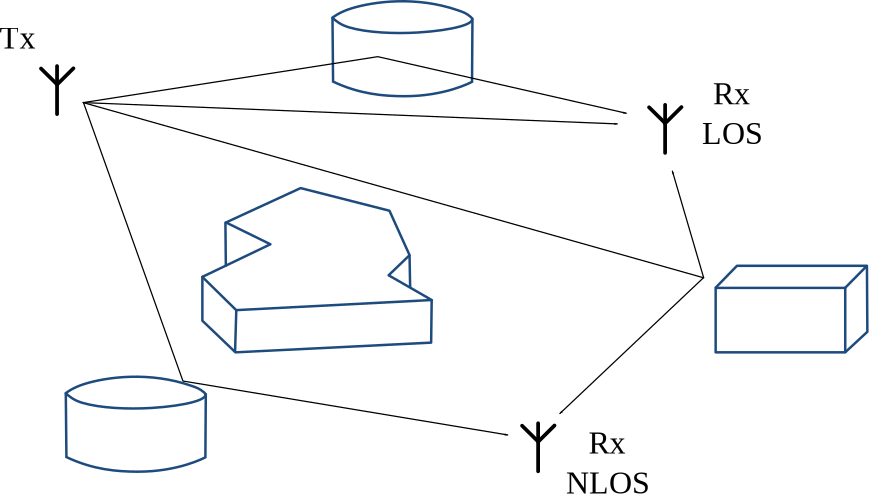
\includegraphics[width=0.9\columnwidth]{figure1}
\caption{Propagazione \textit{Line of Sight} e \textit{Non Line of Sight}.}
\label{fig:1}
\end{figure}
\subsubsection{Propagazione LOS} Vige la legge di Friis del collegamento \cite{Friis} che ci consente di valutare le prestazioni del sistema: $$\frac{P_R}{P_T} = G_T G_R \left ( \frac{\lambda}{4\pi r} \right )^2$$ dove $P_T$ e $P_R$ sono le potenze trasmessa e ricevuta, $G_T$ e $G_R$ i guadagni delle antenne in trasmissione (Tx) e in ricezione (Rx), $\lambda$ la lunghezza d'onda e $r$ la distanza relativa tra Tx e Rx. Sulla base del teorema di Shannon \cite{Shannon1948}, la capacità limite di comunicazione vale in questo caso  $$ C = \log_2(1+\rho_{0}) \ \ \mathrm{[bits/s/Hz]}$$ dove $\rho_0 = \frac{\overline{P_R}}{N_0}$ è il rapporto segnale rumore, con $\overline{P_R}$ la potenza media ricevuta e $N_0$ la potenza di rumore. In ambienti urbani, la componente LOS della propagazione elettromagnetica tende a scomparire, se non per alcuni casi di collegamenti realizzati \textit{ad-hoc} (ponti radio).
\begin{figure}[!ht]
\centering
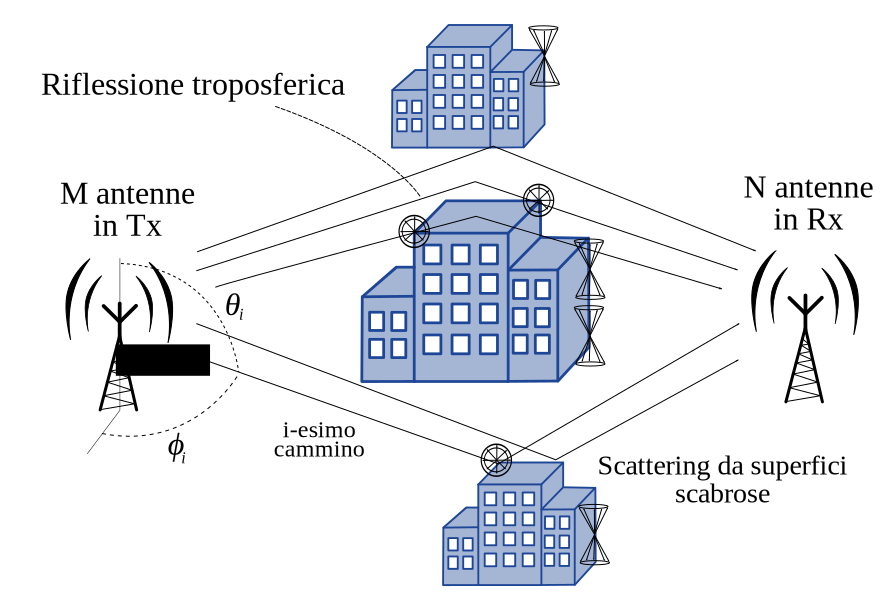
\includegraphics[width=\columnwidth]{figure2}
\caption{Meccanismi di propagazione NLOS.}
\label{fig:2}
\end{figure}
\subsubsection{Propagazione NLOS} È appunto la modalità  di propagazione caratteristica degli ambienti urbani. Le onde trasmesse subiscono riflessione (speculare) e rifrazione (se l'ostacolo risulta trasparente alle frequenze del segnale), diffrazione (da discontinuità  geometriche) e scattering (quando le dimensioni degli ostacoli sono inferiori a $\lambda$ o ad essa paragonabili). Questi fenomeni contribuiscono a degradare le prestazioni della comunicazione, facendo sì che la potenza di segnale ricevuta non sia deterministicamente predicibile entro l'area di copertura. Al ricevitore si sovrappongono onde con sfasamenti differenti relative ai diversi cammini intrapresi dal campo irradiato in Tx, il cosiddetto fenomeno del \textit{multipath}. Particolarmente deleterio è l'annullamento del campo in certi punti dello spazio, portando la potenza di segnale al disotto della soglia di rivelazione del ricevitore. Questo effetto va sotto il nome di \textit{fading} da \textit{multipath}. Per valutare le prestazioni del sistema in questo caso, si deve modellare la propagazione includendo le caratteristiche aleatorie ad essa associate, non essendo deterministici i fenomeni di interazione tra l'onda elettromagnetica e l'ambiente circostante. L'effetto principale della propagazione NLOS è quello di far sì che giungano al ricevitore delle repliche di un simbolo trasmesso ad istanti diversi, dando luogo al \textit{delay spread}. Anche se le repliche che giungono in tempi successivi tendono ad avere energia inferiore (avendo percorso una distanza maggiore), queste si sovrappongono a simboli trasmessi successivamente, con conseguente interferenza intersimbolica. In generale, i meccanismi di propagazione NLOS dipendono dalla frequenza del segnale trasmesso, essendo lo scattering un fenomeno in cui la reirradiazione è funzione delle dimensioni dell'ostacolo in termini di lunghezza d'onda. Si ha scattering alla Rayleigh, pressoché isotropico per oggetti di dimensioni inferiori a $\lambda$ e scattering alla Mie, caratterizzato da una direzione di reirradiazione prevalente, quando le dimensioni dell'ostacolo sono comparabili e maggiori di $\lambda$ \cite{Ishimaru}.




\section{Aspetti fondamentali del MIMO}

\subsection{Diversità spaziale}

\par Il concetto di diversità spaziale \cite{Sarkar} prende spunto dalla considerazione che gli array, disposizione nello spazio di una serie di antenne, consentono di migliorare la risoluzione spaziale, convogliando la potenza entro un determinato angolo solido. Per ottenere una larghezza di fascio più stretta dobbiamo realizzare una distribuzione di antenne sempre più ampia. Nel limite che ci è imposto dall'ingombro risultante, è possibile giungere ad una selettività  spaziale, andando ad isolare delle direzioni di ricetrasmissione. Si può quindi sfruttare, con un sistema ad antenne multiple ed un'opportuna  ``elaborazione spaziale'', le caratteristiche di multipath del canale di propagazione per migliorare le prestazioni del sistema, ossia incrementando il \textit{throughput} (capacità), migliorando l'affidabilità  del collegamento (nei confronti del fading) e riducendo la potenza trasmessa a parità  di prestazioni rispetto ad un sistema a singola antenna.


\subsection{Sistemi radianti per MIMO}

\par In generale, ci si riferisce al sistema radiante in termini di \textit{Multiport Antenna} (MPA). In effetti, il sistema radiante non è necessariamente costituito da una serie di antenne fisicamente distinte, ma può essere realizzato come singola antenna con molteplici porte di alimentazione tali da consentire, a seconda della porta alimentata, una diversa caratteristica di radiazione. Si distinguono quindi tre tipologie di MPA (Fig. \ref{fig:3}-\ref{fig:4}):
\begin{itemize}
\item \textit{Multielement Antenna} (MEA) : un sistema di antenne in cui ciascuna porta è costituita da antenne fisicamente distinte,
\item \textit{Multipolarized Antenna} (MPoA): un sistema di antenne in cui ciascuna porta si riferisce ad una polarizzazione del campo elettrico ben definita,
\item \textit{Multimode Antenna} (MMA): un sistema di antenne in cui ciascuna porta si riferisce ad un pattern di radiazione preciso.
\end{itemize}
\begin{figure}[!h]
\centering
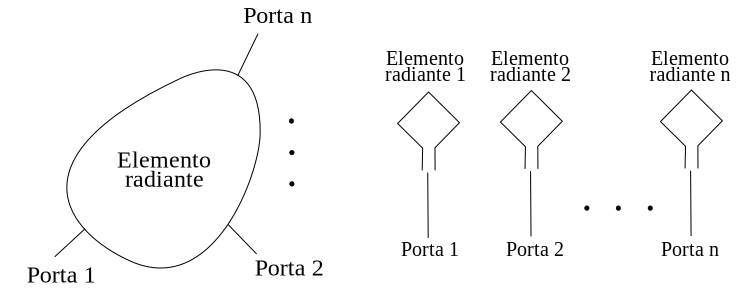
\includegraphics[width=\columnwidth]{figure3}
\caption{Schematizzazione di \textit{Multimode antenna} (sinistra) e \textit{Multielement antenna} (destra).}
\label{fig:3}
\end{figure}
\begin{figure}[!h]
\centering
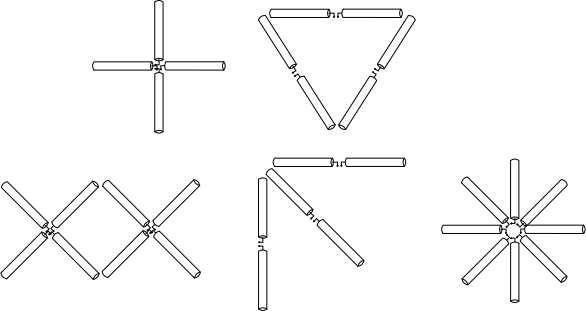
\includegraphics[width=0.9\columnwidth]{figure4}
\caption{Varie conformazioni di \textit{Multipolarized antennas} realizzabili con dipoli.}
\label{fig:4}
\end{figure}




\subsection{Canale MIMO}

\par Si consideri il sistema MIMO $M \times N$ costituito da $M$ porte in trasmissione (\textit{input} nel canale) ed $N$ porte in ricezione (\textit{output} dal canale). Si ha la seguente relazione ingresso-uscita $$\mathbf{r} = \mathbf{H} \mathbf{s} + \mathbf{n}$$ in cui $\mathbf{s} \in \mathbb{C}^{M \times 1}$ è il vettore dei simboli trasmessi, $\mathbf{r} \in \mathbb{C}^{N \times 1}$ i simboli ricevuti, $\mathbf{n} \in \mathbb{C}^{N \times 1}$ le componenti aleatorie del rumore bianco ed $\mathbf{H} \in \mathbb{C}^{N \times M}$ la matrice che caratterizza il canale da un punto di vista elettromagnetico (Fig. \ref{fig:5}).
\begin{figure}[!ht]
\centering

\includegraphics[width=\columnwidth]{figure5}
\caption{Schematizzazione di un sistema MIMO $3 \times 3$ con gli elementi della matrice di canale}
\label{fig:5}
\end{figure}

\par Come discusso nell'introduzione, la propagazione del segnale in un ambiente realistico avviene per collegamenti LOS e NLOS. La matrice di canale, seguendo il medesimo approccio, viene scomposta nella somma di due matrici \cite{Sarris2007}: $$\mat{H} = \sqrt{\frac{K}{1+K}} \overline{\mat{H}} + \sqrt{\frac{1}{1+K}} \widetilde{\mat{H}} $$
dove $\overline{\mat{H}}$ è costituita da variabili deterministiche che descrivono la componente LOS e $\widetilde{\mat{H}}$ è in generale costituita da variabili aleatorie scorrelate con distribuzione gaussiana a valor medio nullo. $K$ è un coefficiente, detto ``riceano'' perché tiene conto della distribuzione di potenza tra LOS e NLOS secondo una statistica di Rice. La distribuzione di Rice modellizza la presenza contemporanea di collegamenti LOS e NLOS, il primo essendo dominante in termini di potenza rispetto all'altro \cite{Lindsey}.

\subsubsection*{Componente $\overline{\mat{H}}$} 
La componente LOS della matrice di canale si valuta assumendo il sistema MIMO posto nello spazio libero come illustrato in Fig. \ref{fig:50}. 

\begin{figure}[!ht]
\centering
\includegraphics[width=.7\columnwidth]{figure50}
\caption{Antenne di un sistema MIMO $3 \times 2$ posto nello spazio libero per la valutazione della componente LOS della matrice di canale.}
\label{fig:50}
\end{figure}

Noti i parametri elettrici delle antenne (diagrammi di radiazione, impedenze) e le distanze relative, $\overline{\mat{H}}$ per un sistema a banda stretta (ipotesi di mezzo non dispersivo) si calcola applicando la formula di Friis ottenendo% \hilight{Dimostrazione in appendice?} 
\begin{eqnarray} 
& & \hspace{-1cm} {\overline {\bf{H}} _{ij}}\left( {{{{\bf{r'}}}_{{T_i}}},{{{\bf{r'}}}_{{R_j}}}} \right) = \nonumber \\ 
& & \hspace{0cm} {K_{R{T_{ij}}}}\Gamma \left( {{r_{ij}}} \right){\left( {{{\bf{F}}^R}\left( {{\Omega _{{R_j}}}} \right)} \right)^\dagger}\,{{\bf{F}}^T}\left( {{\Omega _{{T_i}}}} \right){{\rm{e}}^{ - j{{\bf{k}}_{ij}} \cdot {{\bf{r}}_{ij}}}} \nonumber
\end{eqnarray} con 
\begin{itemize}
\item ${ K_{R{T_{ij}}}} = \sqrt {\frac{{Z_j^{0,R}}}{{Z_i^{0,T}}}} \sqrt {\frac{{\Re \left\{ {Z_i^T} \right\}}}{{\Re \left\{ {Z_j^R} \right\}}}} $, il coefficiente che tiene conto dell'adattamento delle impedenze di uscita delle antenne in Tx e delle impedenze d'ingresso delle antenne in Rx alle rispettive linee di alimentazione,
\item $\Gamma \left( {{r_{ij}}} \right) = \left( {\frac{\lambda }{{4\pi }}} \right){\left( {\frac{1}{{{r_{ij}}}}} \right)^{\frac{{{n_{PL}}}}{2}}}$, il fattore di attenuazione della propagazione (\textit{Path Loss}), ${r_{ij}} = |{{\bf{r'}}_{{T_i}}} - {{\bf{r'}}_{{R_j}}}|$ e ${n_{PL}} \ge 2$,
\item ${{\bf{F}}^T}\left( {{\Omega _{{T_{ij}}}}} \right)$ e ${{\bf{F}}^R}\left( {{\Omega _{{R_{ij}}}}} \right)$, i pattern di radiazione normalizzati, in $\theta$ e $\phi$, rispettivamente nelle direzioni di Tx e di Rx.
\end{itemize} e $\dagger$ evidenzia la relativa matrice trasposta coniugata.
\par Assumendo $\tau _{ij}^0 = \frac{{{r_{ij}}}}{c}$, ossia il ritardo di propagazione tra l'i-esima antenna trasmittente e la j-esima ricevente, la funzione di trasferimento deterministica diventa
\begin{eqnarray} 
& & \hspace{-1cm} {\overline {\bf{H}} _{ij}}\left( {{{{\bf{r'}}}_{{T_i}}},{{{\bf{r'}}}_{{R_j}}}} \right) = \nonumber \\
& & \hspace{0cm} {K_{R{T_{ij}}}}\Gamma \left( {{r_{ij}}} \right){\left( {{{\bf{F}}^R}\left( {{\Omega _{{R_j}}}} \right)} \right)^\dagger}\,{{\bf{F}}^T}\left( {{\Omega _{{T_i}}}} \right){{\rm{e}}^{ - j2\pi f\tau _{ij}^0}}. \nonumber
\end{eqnarray}
%La risposta impulsiva del canale, trasformata inversa di Fourier della funzione di trasferimento, è
%\begin{eqnarray} 
%& & \hspace{-0.8cm} {\overline {\bf{h}} _{ij}}\left( {{{{\bf{r'}}}_{{T_i}}},{{{\bf{r'}}}_{{R_j}}}} \right) = \nonumber \\
%& & \hspace{0cm} {K_{R{T_{ij}}}}\Gamma \left( {{r_{ij}}} \right){\left( {{{\bf{F}}^R}\left( {{\Omega _{{R_j}}}} \right)} \right)^\dagger}\,{{\bf{F}}^T}\left( {{\Omega _{{T_i}}}} \right)\delta \left( {\tau  - \tau _{ij}^0} \right) \nonumber
%\end{eqnarray}

\subsubsection*{Componente $ \widetilde{\mat{H}}$ }
La propagazione NLOS è caratterizzata, in approssimazione deterministica, da una serie cammini ottici o \textit{Multipath Components} (MPC). Per costruire un modello, si ritengono $P$ cammini rilevanti (di potenza ricevuta non trascurabile). Essendo questi cammini considerati deterministici, gli elementi della matrice di canale differiranno da quelle LOS dalla lunghezza del percorso $r_{ij}^p = r_T^p + r_R^p$, dato dalla somma delle distanze tra trasmettitore e diffusore $r_T^p$ e tra diffusore e antenna ricevente $r_R^p$. Vi sarà  inoltre un termine matriciale, la matrice polarimetrica normalizzata ${\bf{C}}_{TR}^p$, che tiene conto dell'interazione tra l'onda elettromagnetica e il diffusore per ciascuna delle componenti $\theta$ e $\phi $. Si ha quindi:
\begin{eqnarray} 
& & \hspace{0cm} {\widetilde {\bf{H}}_{ij}}\left( f, {{{{\bf{r'}}}_{{T_i}}},{{{\bf{r'}}}_{{R_j}}}} \right) = \nonumber \\
& & \hspace{-.8cm} \sum\limits_{p = 1}^P {{K_{R{T_{ij}}}}\Gamma \left( {r_{ij}^p} \right){{\left( {{\bf{F}}_j^R\left( {\Omega _{{R_j}}^p} \right)} \right)}^\dagger}\,{\bf{C}}_{T{R_{ij}}}^p{\bf{F}}_i^T\left( {\Omega _{{T_i}}^p} \right){{\rm{e}}^{ - j2\pi f\tau _{ij}^p}}}. \nonumber
\end{eqnarray}
%La risposta impulsiva associata è quindi
%\begin{eqnarray} 
%& & \hspace{0cm} {\widetilde {\bf{h}}_{ij}}\left( {\tau ,{{{\bf{r'}}}_{{T_i}}},{{{\bf{r'}}}_{{R_j}}}} \right) = \nonumber \\
%& & \hspace{-.8cm} \sum\limits_{p = 1}^P {{K_{R{T_{ij}}}}\Gamma \left( {r_{ij}^p} \right){{\left( {{\bf{F}}_j^R\left( {\Omega _{{R_j}}^p} \right)} \right)}^\dagger}\,{\bf{C}}_{T{R_{ij}}}^p{\bf{F}}_i^T\left( {\Omega _{{T_i}}^p} \right)\delta \left( {\tau  - \tau _{ij}^p} \right)} \nonumber
%\end{eqnarray}
Si noti che l'indice $p = 0$ è riferito alla propagazione LOS, in modo da poter trattare le componenti deterministiche e quelle pseudo-deterministiche (NLOS) rilevanti in un'unica sommatoria. 

\par Per esplicitare la natura aleatoria della propagazione NLOS, vi sono sostanzialmente tre modelli statistici:
\begin{itemize}
\item il \textit{modello Kronecker}, che assume scorrelati i processi di fading tra Tx e Rx. Si appoggia sulla valutazione di matrici di correlazione spaziale tra le antenne del trasmettitore e analogamente tra quelle del ricevitore. Viene in particolare usato dallo standard l'IEEE 802.11n per implementare la codifica MIMO \cite{IEEE80211n},
\item il \textit{modello Weichselberger}, che consente di considerare i processi di fading tra Tx e Rx non scorrelati. I suoi parametri principali sono gli autovettori delle matrici di correlazione ed una matrice di accoppiamento diretto tra Tx e Rx,
\item la \textit{rappresentazione virtuale di canale}, che è analoga al modello Weichselberger ma impiega i vettori di eccitazione delle porte, riferendosi quindi allo spazio di pattern (il passaggio dalle eccitazioni al pattern è sostanzialmente una trasformata di Fourier \cite{Balanis}), invece degli autovettori delle matrici di correlazione.
\end{itemize}

\subsection{Propagazione ricca di scattering}
Il modello Kronecker è il più popolare per la sua semplicità  analitica e la rispondenza per gli ambienti ricchi di scattering. Essendo le antenne in Tx e Rx scorrelate, la matrice di canale NLOS può essere riscritta nella forma
\[\widetilde {\bf{H}} = {\left( {{\bf{R}}_H^R} \right)^{\frac{1}{2}}}{\bf{W}}{\left( {{{\left( {{\bf{R}}_H^T} \right)}^{\frac{1}{2}}}} \right)^\dagger}\]
dove ${\bf{W}} \in \mathbb{C}{^{N \times M}}$ è una matrice i cui elementi sono variabili aleatorie distribuite $N(0,1)$ (distribuzione gaussiana a media nulla e varianza unitaria), ${\bf{R}}_H^T \in \mathbb{C}{^{M \times M}}$ e ${\bf{R}}_H^R \in \mathbb{C}{^{N \times N}}$ sono rispettivamente le matrici di correlazione spaziale in Tx e Rx. Quest'ultime si possono ricavare da una campagna di misure di canale dalle relazioni
\[{\bf{R}}_H^T = \frac{{E\left\{ {{{\left( {\widetilde {\bf{H}}} \right)}^\dagger}\widetilde {\bf{H}}} \right\}}}{{\sqrt {E\left\{ {\left\| {\widetilde {\bf{H}}} \right\|_F^2} \right\}} }} \qquad {\bf{R}}_H^R = \frac{{E\left\{ {\widetilde {\bf{H}}{{\left( {\widetilde {\bf{H}}} \right)}^\dagger}} \right\}}}{{\sqrt {E\left\{ {\left\| {\widetilde {\bf{H}}} \right\|_F^2} \right\}} }}\,\,\] dove $\| \|_F$ è la norma di Frobenius e $E\{\cdot\}$ il valore atteso.
Si definisce la correlazione di canale ${\mathcal{R}^H}$ come la covarianza della vettorializzazione (le colonne della matrice vengono concatenate in un'unica colonna con l'operatore $\mathrm{vec}(\cdot)$) della matrice di canale NLOS oppure come il prodotto di Kronecker ($\otimes$) tra le matrici di correlazione Tx e Rx
\[{\mathcal{R}^H} = E\left\{ {{\rm{vec}}\left( {\widetilde {\bf{H}}} \right){\rm{vec}}{{\left( {\widetilde {\bf{H}}} \right)}^\dagger}} \right\} = {\bf{R}}_H^T \otimes {\bf{R}}_H^R\]
Le matrici di correlazione possono inoltre essere valutate analiticamente dai pattern di radiazione normalizzati con:
\[{\bf{R}}_{{H_{ij}}}^{R,T} = \frac{{{\bf{X}}_{{H_{ij}}}^{R,T}}}{{\sqrt {{\bf{X}}_{{H_{ii}}}^{R,T}{\bf{X}}_{{H_{jj}}}^{R,T}} }}\]
\[{\bf{X}}_{{H_{ij}}}^{R,T} = \frac{1}{{8\pi }}\int\limits_{ - \pi }^\pi  {\int\limits_0^\pi  {{{\left( {{\bf{F}}_i^{R,T}\left( {\theta ,\phi } \right)} \right)}^\dagger}{\bf{F}}_j^{R,T}\left( {\theta ,\phi } \right)} } \sin \left( \theta  \right)d\theta d\phi \]
dove ${\bf{X}}_{{H_{ij}}}^{R,T}$ sono termini di covarianza relativi alle porte del ricevitore o del trasmettitore. 
\par Siamo in generale interessati a valutare le prestazioni di un sistema MIMO in ambiente ricco di scattering, il canale verrà quindi nel seguito assunto esclusivamente caratterizzato da propagazione NLOS, ossia ${\bf{H}} \approx \widetilde {\bf{H}}$ (coefficiente riceano $K = 0$). Si noti inoltre che la componente LOS è tale da aumentare la correlazione \cite{Sarris2007} tra i vari cammini del canale, peggiorando quindi le prestazioni del sistema MIMO.


\subsection{Normalizzazione della matrice di canale} 

Per poter confrontare le prestazioni di diversi sistemi multiantenna, è opportuno procedere con una normalizzazione del canale, assumendo come riferimento la potenza ricevuta $P_R$. A seguito della normalizzazione, la capacità  di canale diventa una funzione del rapporto segnale rumore (\textit{Signal to Noise Ratio} o SNR) $\rho_0$ al ricevitore mediato nel tempo su tutte le porte \cite{Jensen, Gesbert}
\[C = {\log _2}\det \left( {{\bf{I}} + \frac{{{\rho _0}}}{M}{{\bf{H}}_0}{\bf{H}}_0^\dagger} \right)\]

\par Si considerino $Q$ realizzazioni diverse di canale (diverse disposizioni del trasmettitore e del ricevitore nello spazio) per un'analisi delle variazioni relative allo spostamento di un terminale ricetrasmittente mobile. La matrice di canale normalizzata della q-esima realizzazione si ottiene con la seguente
\[{\bf{H}}_0^q = {{\bf{H}}^q}\sqrt {\frac{{NMQ}}{{\sum\nolimits_{q = 1}^Q {\left\| {{{\bf{H}}^q}} \right\|_F^2} }}} \]

\par Utilizzando il modello di Kronecker per il canale, si giunge alla seguente relazione per la capacità  di canale
\[C = {\log _2}\det \left( {{\bf{I}} + \frac{{{\rho _0}}}{M}{\bf{R}}_{{{\bf{H}}_0}}^R{\bf{WR}}_{{{\bf{H}}_0}}^T{{\bf{W}}^\dagger}} \right)\]
da cui si intuisce che per massimizzare la capacità  di sistema occorre realizzare sistemi di antenne tali per cui le $M$ porte in Tx siano scorrelate tra di loro,  e ad egual modo per le $N$ porte in Rx:
\[{\bf{R}}_{{{\bf{H}}_0}}^{R,T} \to {\bf{I}}\]
In tal caso le  prestazioni del sistema non dipendono più dal particolare MPA usato e le porte si dicono scorrelate.
Questo risultato si può ottenere andando a minimizzare gli accoppiamenti mutui tra le antenne oppure realizzando delle reti di decorrelazione.

\subsection{\textit{Clusters}}

In generale, i cammini di propagazione NLOS (MPC) non sono determinati univocamente. Si preferisce raggrupparli in \textit{clusters} in trasmissione (in ricezione), ossia un gruppo di cammini provenienti dal trasmettitore (diretti al ricevitore) entro un certo angolo solido e che giungono in modo diverso al ricevitore (che provengono in modo diverso dal trasmettitore). Ci si aspetta che più stretto è l'angolo solido associato ad un {cluster}, minore sarà il ritardo associato al \textit{delay spread}. Il \textit{delay spread} viene modellato con una funzione di dispersione (esponenziale decrescente) che moltiplica la matrice polarimetrica normalizzata relativa ad un {cluster}.

\begin{figure}[!ht]
\centering
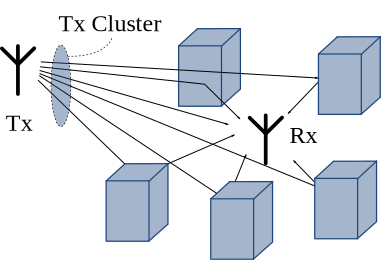
\includegraphics[width=.55\columnwidth]{figure7}
\caption{\textit{Cluster} in trasmissione.}
\label{fig:7}
\end{figure}

\subsection{Distribuzione spaziale di $P_R$}

La variazione della distanza relativa tra Tx e Rx influenza notevolmente la potenza di segnale ricevuto, quindi la capacità  media del sistema. Si individuano tre componenti relative alla variazione di $P_R$ (Fig. \ref{fig:8}):
\begin{itemize}
\item Le \textit{path losses}, inversamente proporzionali alla distanza tra Tx e Rx secondo l'esponente ${n_{PL}} \ge 2$,
\item Il {fading} lento, fluttuazioni su larga scala circa ogni $10 \lambda$,
\item Il {fading} rapido, fluttuazioni su scala microscopica circa ogni $\lambda$.
\end{itemize}

\begin{figure}[!h]
\centering
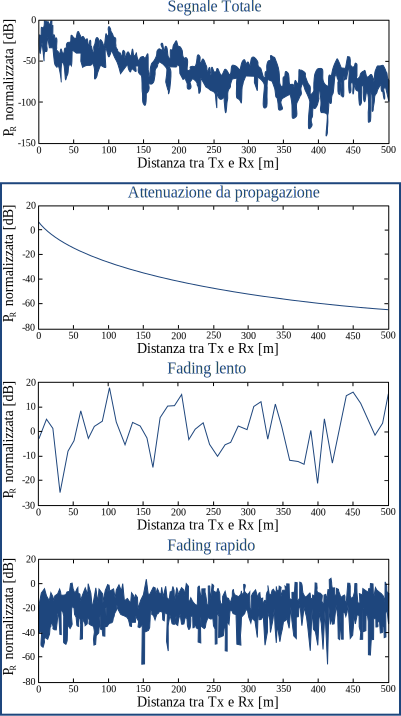
\includegraphics[width=.8\columnwidth]{figure8}
\caption{Andamento di $P_R$ al variare della distanza tra Tx e Rx \cite{DeFlavis}.}
\label{fig:8}
\end{figure}

\subsection{Tecniche di codifica MIMO}

\par Vi sono sostanzialmente tre tecniche di codifica MIMO:
\subsubsection{Tecniche di diversità  spaziale o Space-Time Coding (STC)} vengono usate per aumentare la  potenza di segnale dei simboli ricevuti, quindi ad incrementare l'SNR \cite{SmartAntennas}. Si ha ridondanza dei simboli inviati da antenne diverse, consentendo quindi di combattere il {fading} rapido. Tra i parametri di riferimento vi è il guadagno di diversità o ordine di diversità ${G_d} =  - \mathop {\lim }\limits_{\gamma  \to \infty } \frac{{\log {P_e}}}{{\log \gamma }}$ con $P_e$ la probabilità  di errore e $\gamma$ l'SNR (Fig. \ref{fig:9}). Per un sistema MIMO $M \times N$, ${G_d}$ vale al massimo $MN$.
\begin{figure}[!h]
\centering
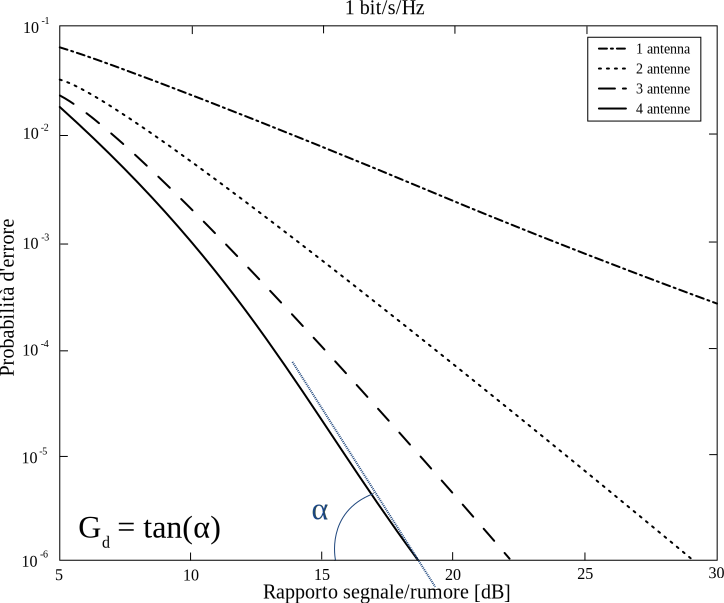
\includegraphics[width=0.95\columnwidth]{figure9}
\caption{Andamento della probabilità di errore rispetto all'SNR per un sistema STC al variare del numero di antenne in ricezione.}
\label{fig:9}
\end{figure}

\subsubsection{Multiplazione spaziale (SM)} è una tecnica che aumenta il {throughput} di comunicazione. Si inviano simboli diversi contemporaneamente e con la medesima portante ma tramite antenne diverse. Si ha il guadagno di multiplazione ${G_{sm}} = \mathop {\lim }\limits_{\gamma  \to \infty } \frac{R}{{\log \gamma }}$ con $R$ il rate dei simboli e $\gamma$ l'SNR. Per un sistema MIMO $M \times N$, ${G_{sm}}$ vale al massimo $\min (M,N)$, ossia il numero massimo di cammini indipendenti effettivi.

\subsubsection{Tecniche di Beamforming} è una tecnica usata per aumentare sia la potenza di segnale che il rate di trasmissione \cite{Baumgartner}. Il guadagno d'array \cite{Balanis} dovuto alla combinazione coerente (tramite reti di \textit{beamforming} o BFN) dei segnali sulle antenne in Tx o Rx è tale da migliorare l'SNR in ricezione, quindi la capacità di sistema. % Richiede la conoscenza del canale di propagazione sia da parte del trasmettitore che del ricevitore.
Si va quindi ad amplificare il segnale relativo ad un determinato {cluster}.
\begin{figure}[!ht]
\centering
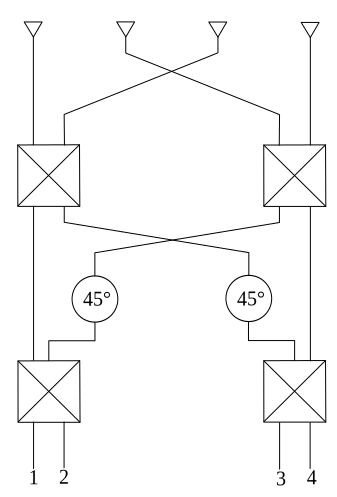
\includegraphics[width=0.6\columnwidth]{figure10}
\caption{Esempio di rete di \textit{beamforming}: la ``matrice di Butler''.}
\label{fig:10}
\end{figure}

\begin{figure}[!ht]
\centering
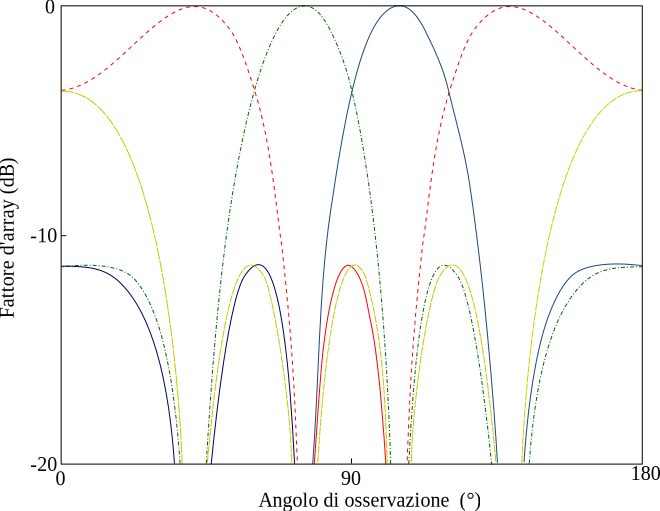
\includegraphics[width=0.95\columnwidth]{figure11}
\caption{Guadagni normalizzati ottenibili dalla matrice di Butler di Fig. \ref{fig:10} a seconda della porta di eccitazione.}
\label{fig:11}
\end{figure}

\section{Modello per sistemi MIMO}

\par È ben noto che una collocazione ravvicinata di antenne dà luogo ad accoppiamenti mutui. Le caratteristiche elettriche proprie delle antenne variano (pattern di radiazione, impedenza d'ingresso) per la presenza delle antenne circostanti (così come varia il comportamento di un'antenna dallo spazio libero di progetto all'ambiente operativo reale). Le antenne di un MPA non possono quindi essere considerate indipendenti l'una dall'altra. Caratterizzando la radiazione di un sistema ad antenne multiple in termini di armoniche sferiche (set di pattern di radiazione ortonormali derivati dalla soluzione dell'equazione di Laplace in coordinate sferiche), si può caratterizzare l'interazione tra le onde guidate e quelle radiate in termini di parametri di scattering.
\begin{figure}[!ht]
\centering
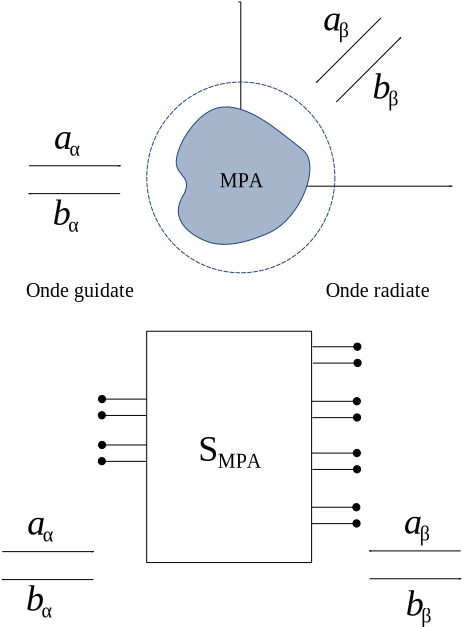
\includegraphics[width=0.7\columnwidth]{figure12}
\caption{MPA e rappresentazione modale della propagazione elettromagnetica guidata e radiata.}
\label{fig:12}
\end{figure} Troncando il numero di armoniche sferiche (insieme infinito) ai modi rilevanti (di potenza non trascurabile), possiamo scrivere
\begin{eqnarray}
& & \hspace{-1.5cm} {{\bf{b}}^{T,R}} = \left( {\begin{array}{*{20}{c}} {{\bf{b}}_\alpha ^{T,R}}\\ {{\bf{b}}_\beta ^{T,R}} \end{array}} \right) \nonumber \\
& & \hspace{-1cm} = \left( {\begin{array}{*{20}{c}}
{{\bf{S}}_{\alpha \alpha }^{T,R}}&{{\bf{S}}_{\alpha \beta }^{T,R}}\\
{{\bf{S}}_{\beta \alpha }^{T,R}}&{{\bf{S}}_{\beta \beta }^{T,R}}
\end{array}} \right)\left( {\begin{array}{*{20}{c}}
{{\bf{a}}_\alpha ^{T,R}}\\
{{\bf{a}}_\beta ^{T,R}}
\end{array}} \right) = {{\bf{S}}^{T,R}}{{\bf{a}}^{T,R}} \nonumber
\end{eqnarray} dove ${\bf{S}}_{\alpha \alpha }^{T,R}$ è la matrice di scattering che tiene conto delle riflessioni e degli accoppiamenti mutui, ${\bf{S}}_{\alpha \beta }^{T,R},{\bf{S}}_{\beta \alpha }^{T,R}$ rappresentano i pattern di radiazione modali in Tx e Rx e ${\bf{S}}_{\beta \beta }^{T,R}$ è il campo diffuso dall'antenna (la quale potenza non risulta disponibile ai morsetti dell'antenna). Il pedice $\alpha$ si riferisce alla propagazione guidata, mentre $\beta$ a quella radiata. Il pattern associato alla i-esima porta è dato dalla serie:
\[{\bf{F}}_i^{R,T}\left( {\theta ,\phi } \right) = \sum\limits_{j = 1}^\infty  {{\bf{S}}_{{\beta}{\alpha_ji}}^{R,T}{{\bf{\Psi }}_j}\left( {\theta ,\phi } \right)} \]
dove ${{\bf{\Psi }}_j}\left( {\theta ,\phi } \right)$ sono le funzioni modali ortonormali dell'espansione in armoniche sferiche. Per antenne prive di perdite, possiamo scrivere \cite{Was2005}
\begin{eqnarray}
\label{eq:patternOrtogonalization}
& & \hspace{-1cm} \int\limits_{ - \pi }^\pi  {\int\limits_0^\pi  {{{\left( {{\bf{F}}_i^{R,T}\left( {\theta ,\phi } \right)} \right)}^\dagger}{\bf{F}}_i^{R,T}\left( {\theta ,\phi } \right)} } \sin \left( \theta  \right)d\theta d\phi = \nonumber \\ 
& & {\left( {{\bf{S}}_{\beta {\alpha _{*i}}}^{R,T}} \right)^\dagger}{\bf{S}}_{\beta {\alpha _{*i}}}^{R,T} \le {\bf{I}} - {\left( {{\bf{S}}_{\alpha {\alpha _{*i}}}^{R,T}} \right)^\dagger}{\bf{S}}_{\alpha {\alpha _{*i}}}^{R,T}
\end{eqnarray} dove ${\bf{S}}_{\alpha {\alpha _{*i}}}^{R,T}$ è l'i-esima colonna di ${\bf{S}}_{\alpha \alpha }^{R,T}$. La potenza irradiata è data da:
\begin{eqnarray}
& & \hspace{-1cm} \overline{P_{{\alpha _T}}^{T}} = {\left( {{\bf{b}}_{{\beta _T}}^T} \right)^\dagger}{\bf{b}}_{{\beta _T}}^T = {\left( {{\bf{a}}_{{\beta _T}}^T} \right)^\dagger}{\left( {{\bf{S}}_{{\beta _T}{\alpha _T}}^T} \right)^\dagger}{\bf{S}}_{{\beta _T}{\alpha _T}}^T{\bf{a}}_{{\alpha _T}}^T \nonumber \\
& & \le {\left( {{\bf{a}}_{{\beta _T}}^T} \right)^\dagger}\left( {{\bf{I}} - {{\left( {{\bf{S}}_{{\alpha _T}{\alpha _T}}^T} \right)}^\dagger}{\bf{S}}_{{\alpha _T}{\alpha _T}}^T} \right){\bf{a}}_{{\alpha _T}}^T \nonumber
\end{eqnarray} Per la reciprocità delle antenne, risultati analoghi si ottengono per la potenza media in ricezione.

\par L'intero sistema MIMO viene scomposto sostanzialmente in tre blocchi: l'MPA in Tx, il canale di propagazione e l'MPA in Rx (Fig. \ref{fig:13}). Il comportamento elettromagnetico dei vari blocchi viene caratterizzato con matrici di scattering.
\begin{figure}[!ht]
\centering
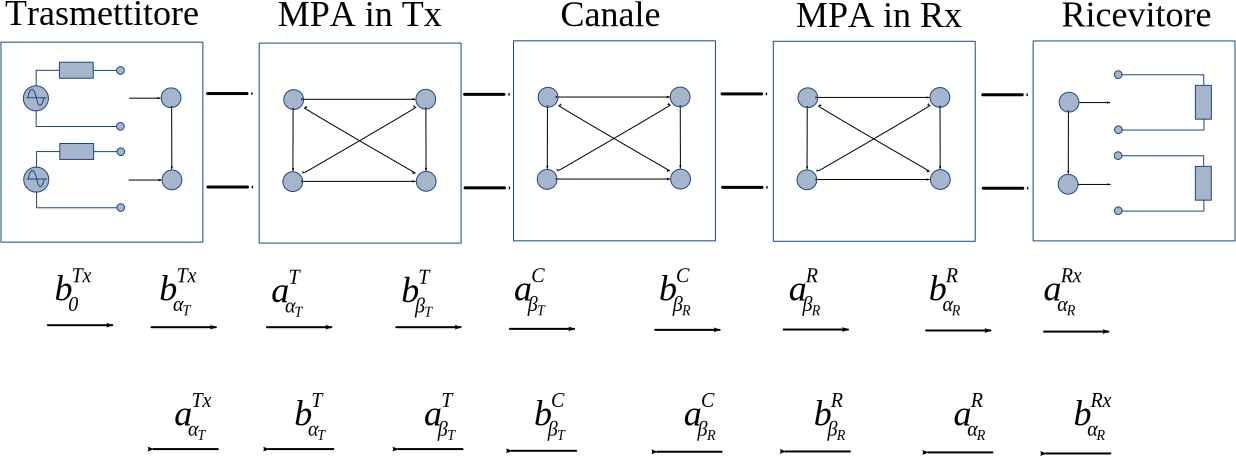
\includegraphics[width=\columnwidth]{figure13}
\caption{Schema a blocchi di un generico sistema MIMO.}
\label{fig:13}
\end{figure}
Valutata la matrice di ciascun blocco, si costruisce per concatenazione ($\odot$) delle matrici di scattering la matrice estesa del canale MIMO (Fig. \ref{fig:14}):
\[{{\bf{S}}^E} = {{\bf{S}}^T} \odot {{\bf{S}}^C} \odot {{\bf{S}}^R}\]
\begin{figure}[!ht]
\centering
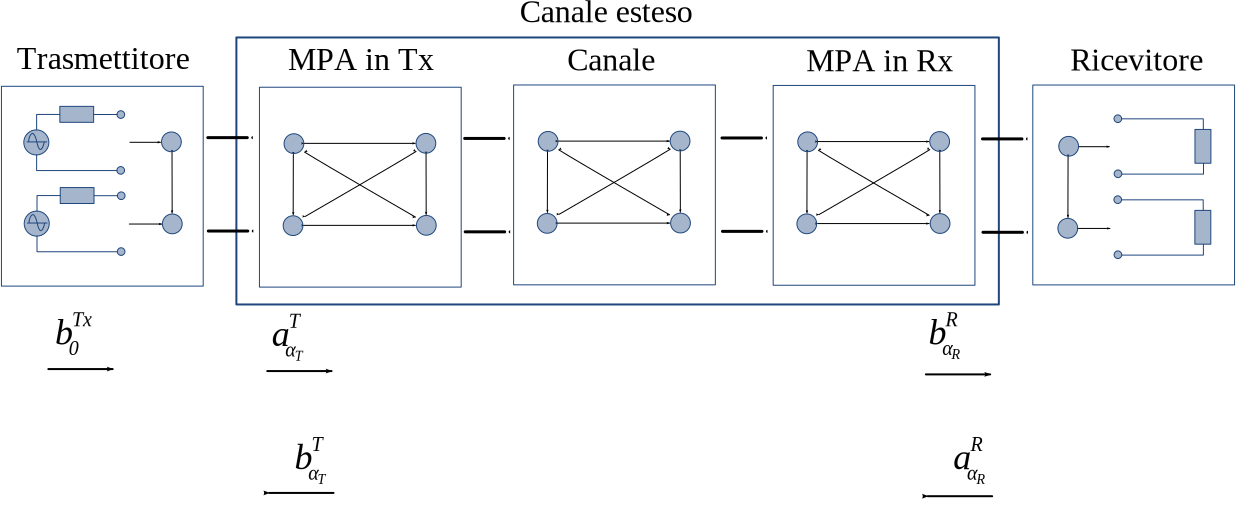
\includegraphics[width=\columnwidth]{figure14}
\caption{Matrice di canale estesa.}
\label{fig:14}
\end{figure}
Per semplificare la costruzione della matrice di scattering estesa, si assume il canale adattato (${\bf{S}}_{{\beta _T}{\beta _T}}^C = 0$ e ${\bf{S}}_{{\beta _R}{\beta _R}}^C = 0$), ossia che a livello delle transizioni tra antenna ed aria tutta la potenza venga trasferita (si sono inclusi tutti i modi sferici rilevanti e non vi sono perdite) e che la propagazione sia unilaterale (${\bf{S}}_{{\beta _T}{\beta _R}}^C = 0$), da Tx a Rx. La matrice estesa risultante è 

\begin{eqnarray}
{{\bf{S}}^E} & = & \left( {\begin{array}{*{20}{c}} {{\bf{S}}_{{\alpha_T}{\alpha _T}}^T}&{\bf{0}}\\ {{\bf{S}}_{{\alpha_R}{\beta_R}}^R{\bf{S}}_{{\beta_R}{\beta_T}}^C{\bf{S}}_{{\beta_T}{\alpha_T}}^T}&{{\bf{S}}_{{\alpha_R}{\alpha_R}}^R}\end{array}} \right) \nonumber \\
& = & \left( {\begin{array}{*{20}{c}} {{\bf{S}}_{{\alpha _T}{\alpha _T}}^T}&{\bf{0}}\\ {\bf{H}}&{{\bf{S}}_{{\alpha _R}{\alpha _R}}^R} \end{array}} \right) \nonumber
\end{eqnarray} La matrice $N \times M$ data dal prodotto ${\bf{S}}_{{\alpha _R}{\beta _R}}^R{\bf{S}}_{{\beta _R}{\beta _T}}^C{\bf{S}}_{{\beta _T}{\alpha _T}}^T$ descrive la trasmissione di segnali dalle porte di Tx a quelle di Rx. È quindi la matrice di canale che lega le $M$ porte in trasmissione alle $N$ porte in ricezione.

\subsection{Matrice estesa e modello Kronecker}

\par Per valutare le prestazioni di un sistema MIMO è possibile separare il trasmettitore dal ricevitore (Fig. \ref{fig:15}), valutandone le prestazioni individuali separatamente. Quest'approccio è particolarmente utile quando l'ambiente è ricco di scattering, ed il modello Kronecker viene usato per la matrice di canale.
\begin{figure}[!h]
\centering
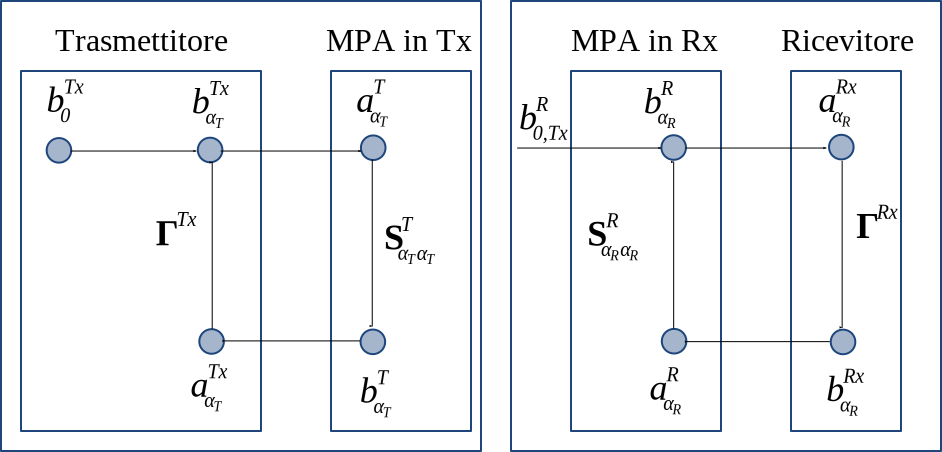
\includegraphics[width=.9\columnwidth]{figure15}
\caption{Separazione delle antenne in Tx da quelle in Rx nel modello MIMO a parametri di scattering.}
\label{fig:15}
\end{figure}
\par L'analisi si riconduce quindi alla valutazione delle interazioni dirette tra le porte di un MPA, evidenziate dalle sottomatrici ${{\bf{S}}_{{\alpha _T}{\alpha _T}}^T}$ e ${{\bf{S}}_{{\alpha _R}{\alpha _R}}^R}$ della matrice estesa. Queste interazioni vanno sotto il nome di mutui accoppiamenti ed avvengono sostanzialmente per tre meccanismi (Fig. \ref{fig:16}):
\begin{itemize}
\item accoppiamenti diretti tra gli elementi,
\item onde superficiali nel dielettrico di supporto per antenne planari,
\item riflessioni e scattering in campo vicino da oggetti metallici circostanti.
\end{itemize}
\begin{figure}[!h]
\centering
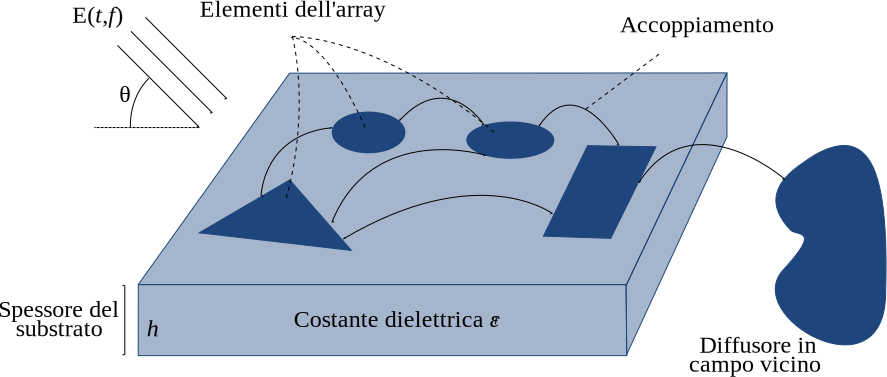
\includegraphics[width=0.9\columnwidth]{figure16}
\caption{Fenomeno dei mutui accoppiamenti tra antenne e cause principali.}
\label{fig:16} 
\end{figure} 
La matrice ${{\bf{S}}_{{\alpha_{T,R}}{\alpha_{T,R}}}^{T,R}}$ si ottiene con la seguente tecnica: eccitando un'antenna per volta e chiudendo le altre su carichi adattati, si misura il coefficiente di riflessione alla porta alimentata. Una misura della potenza dissipata dai carichi delle altre antenne consente di calcolare, nota anche la potenza erogata dalla sorgente, il coefficiente di accoppiamento (Fig. \ref{fig:17}).
\begin{figure}[!h]
\centering
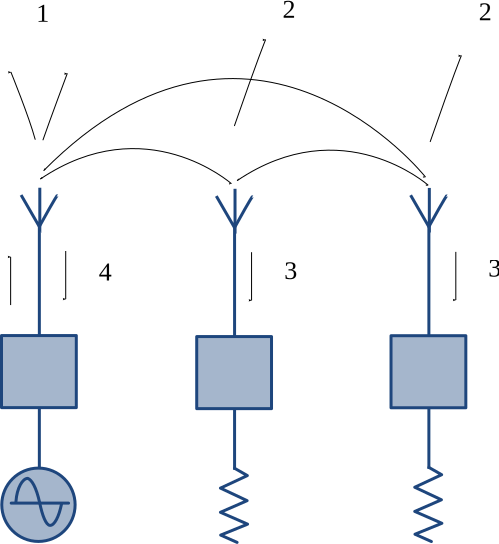
\includegraphics[width=0.5\columnwidth]{figure17}
\caption{Meccanismi fisici in un MPA: 1. Radiazione, 2. Scattering da elementi non eccitati, 3. Potenza accoppiata, 4. Potenza riflessa }
\label{fig:17}
\end{figure} 

\par I parametri che permettono di caratterizzare il sistema MIMO sono:
\begin{itemize}
\item il guadagno di trasmissione di potenza nell'intera catena da Tx a Rx:
\begin{eqnarray}
{G_{tp}} = \frac{{{P_R}}}{{{P_T}}} & = & G_{tp}^TG_{tp}^CG_{tp}^R \nonumber \\
& = & \frac{{{{\left( {{\bf{b}}_{{\alpha _R}}^R} \right)}^\dagger}{\bf{b}}_{{\alpha _R}}^R - {{\left( {{\bf{a}}_{{\alpha _R}}^R} \right)}^\dagger}{\bf{a}}_{{\alpha _R}}^R}}{{{{\left( {{\bf{a}}_{{\alpha _T}}^T} \right)}^\dagger}{\bf{a}}_{{\alpha _T}}^T - {{\left( {{\bf{b}}_{{\alpha _T}}^T} \right)}^\dagger}{\bf{b}}_{{\alpha _T}}^T}} \nonumber
\end{eqnarray}
\item la correlazione del canale esteso ${\mathcal{R}^E} = {\bf{R}}_E^T \otimes {\bf{R}}_E^R$,
\item la correlazione estesa tra antenne ${\bf{X}}_E^{R,T}$. Nel caso particolare di antenne adattate all'impedenza caratteristica di linea si ha ${\bf{\Gamma }}_{{\alpha _R}}^D = {\bf{0}}$, quindi ${\bf{X}}_E^{R,T} = {\bf{X}}_H^{R,T}$,
\item la capacità  di sistema
\begin{equation}
\label{eq:capacita}
C = {\log _2}\det \left( {{\bf{I}} + \frac{{{\rho _0}}}{M}{\bf{R}}_{{{\bf{E}}_0}}^R{\bf{WR}}_{{{\bf{E}}_0}}^T{{\bf{W}}^\dagger}} \right),
\end{equation} 
\item il guadagno di diversità  ${G_d} = \mathrm{rank}\left( {{\bf{R}}_{{{\bf{E}}_0}}^T} \right)\,\mathrm{rank}\left( {{\bf{R}}_{{{\bf{E}}_0}}^R} \right)$,
\item la banda $B$, valutata sui coefficienti di riflessione (condizioni più stringenti) alla sorgente e al carico, tipicamente a – 6 dB (75 \% di efficienza),
\item i gradi di libertà (spaziale) effettivi o \textit{Effective Degrees of Freedom} $$ EDoF\,\, = \,\,{\left. {\frac{{\partial C\left( x \right)}}{{\partial {{\log }_2}\left( x \right)}}} \right|_{x = \rho }},$$ che tende a $\min \left( {M,N} \right)$ all'aumentare dell'SNR.
\end{itemize}

\section{Progetto di antenne per MIMO}

\par Il progetto di antenne per sistemi MIMO si basa sul principio che un aumento del numero di antenne (quindi del costo complessivo dell'apparecchiatura) deve tradursi in un effettivo miglioramento delle prestazioni, in particolare di un aumento della capacità. L'aumento di capacità \eqref{eq:capacita} si può ottenere, come visto in precedenza, andando a massimizzare il guadagno di trasmissione di potenza, il quale massimizza appunto l'SNR al ricevitore. Assumendo la propagazione ricca di scattering (modello Kronecker), si deve realizzare una condizione di ``adattamento coniugato multiporta'' tra le $M$ sorgenti e l'MPA in Tx e tra l'MPA in Rx e i carichi (impedenze d'ingresso dei ricevitori), implementando le condizioni
\[\begin{array}{l}
{{\bf{\Gamma }}^{Tx}} = {\left( {{\bf{S}}_{{\alpha _T}{\alpha _T}}^T} \right)^\dagger},\\
{{\bf{\Gamma }}^{Rx}} = {\left( {{\bf{S}}_{{\alpha _R}{\alpha _R}}^R} \right)^\dagger}.
\end{array}\]
\par Inoltre, per aumentare la capacità, si deve minimizzare la correlazione di canale (assicurandosi dell'effettiva ricchezza di scattering) e la correlazione tra le antenne (riducendo gli accoppiamenti mutui). Tra le tecniche disponibili per minimizzare la correlazione, si hanno
\begin{itemize}
\item l'implementazione di un efficace diversità di antenna (spaziale, di polarizzazione, di pattern),
\item l'impiego di reti di decorrelazione (\textit{Decorrelating Networks} o DNs),
\end{itemize}
le quali vanno prevalentemente ad agire sulla correlazione tra antenne riducendo i mutui accoppiamenti.% Si noti che il progetto di DNs, essendo tipicamente basato su condizioni di propagazione NLOS ideali, richiede un meticoloso riadattamento del sistema a condizioni reali. Le DNs sono particolarmente difficili da realizzare in quanto sono progettate per ambienti NLOS ideali.

\par Analiticamente, per avere disaccoppiamento tra le antenne in un MPA si deve avere
\[\int\limits_{ - \pi }^\pi  {\int\limits_0^\pi  {{{\left( {{\bf{F}}_i^{R,T}\left( {\theta ,\phi } \right)} \right)}^\dagger}{\bf{F}}_i^{R,T}\left( {\theta ,\phi } \right)} } \sin \left( \theta  \right)d\theta d\phi \,\, = \,\,{\bf{I}},\]
quindi, da \eqref{eq:patternOrtogonalization}, ${\left( {{\bf{S}}_{\alpha \alpha }^{R,T}} \right)^\dagger}{\bf{S}}_{\alpha \alpha }^{R,T} = {\bf{0}}$ ovvero ${\bf{S}}_{\alpha \alpha }^{R,T} = {\bf{0}}$. Da un punto di vista della matrice estesa, le matrici di scattering diagonali devono annullarsi (${\bf{S}}_{{\alpha _{R,T}}{\alpha _{R,T}}}^{R,T} = {\bf{0}}$). In conclusione, pattern ortogonali implicano porte scorrelate agli MPA. Da un punto di vista elettromagnetico, pattern ortogonali si ottengono con la diversità spaziale, ossia con antenne identiche distanziate opportunamente, con la diversità di polarizzazione, ovvero con antenne polarizzate diversamente e con la diversità di pattern, cioè da angoli solidi di ricetrasmissione distinti.

\subsection{Diversità di antenna}

\subsubsection{Diversità  spaziale}
\par Un criterio progettuale per distanziare gli elementi di un MEA di antenne è dato dal modello di Jakes \cite{DeFlavis} per la correlazione tra due antenne isotrope con una distribuzione uniforme d'incidenza azimutale (2D) rappresentazione dalla relazione
\[{{\bf{R}}_{{H_{ij}}}} = {J_0}\left( {k{d_{ij}}} \right),\]
che lega la correlazione tra le antenne alla loro distanza relativa secondo una funzione di Bessel del primo tipo e di ordine 0 (Fig. \ref{fig:18}). Tipicamente si sceglie ${d_{ij}} \ge \frac{\lambda }{2}$.
\begin{figure}[h]
\centering
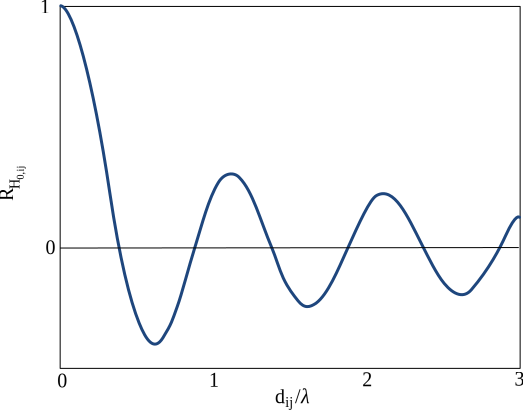
\includegraphics[width=0.6\columnwidth]{figure18}
\caption{Coefficiente di correlazione spaziale al variare della distanza tra antenne antenne isotropiche equipolarizzate.}
\label{fig:18}
\end{figure}

%\begin{figure}[!ht]
%\centering
%\includegraphics[width=\columnwidth]{figure19}
%\caption{}
%\label{fig:19}
%\end{figure}
\par Come si evince dalla Fig. \ref{fig:20}, anche la modalità di propagazione influenza notevolmente il coefficiente di correlazione, e limitarsi a considerare un ambiente ideale ricco di scattering può essere sinonimo di cattivo progetto.
\begin{figure}[h]
\centering
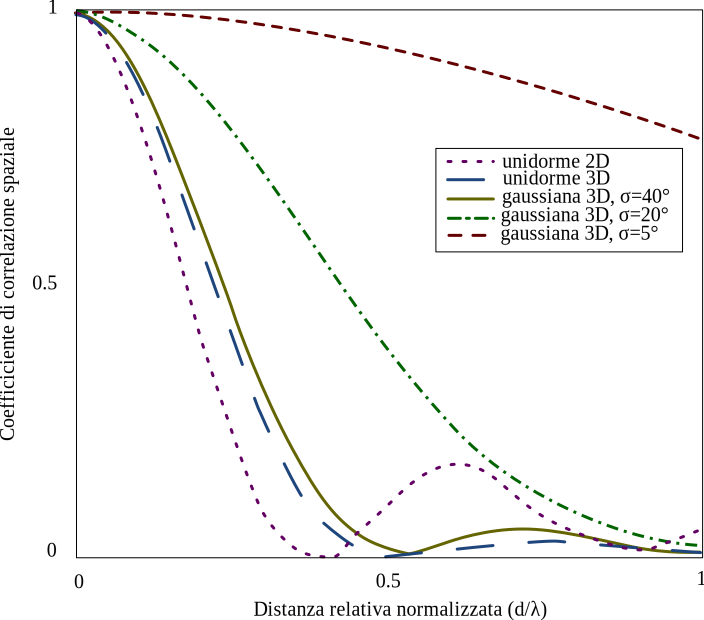
\includegraphics[width=0.9\columnwidth]{figure20}
\caption{Andamento del coefficiente di correlazione spaziale al variare della distanza relativa tra due antenne a patch, trascurando gli effetti dei mutui accoppiamenti. Le curve sono relative a diverse distribuzioni assunte per l'angolo solido di osservazione (tratto da \cite{Ozdemir2004}).}
\label{fig:20}
\end{figure}

\subsubsection{Diversità  di polarizzazione}

\par Le antenne sono disposte in modo da corrispondere ad una determinata polarizzazione del campo \cite{Zhang, Das2004}. In Fig. \ref{fig:52} vi è un esempio di MPoA realizzato con tre dipoli stampati \cite{Chui2007}.
\begin{figure}[h]
\centering
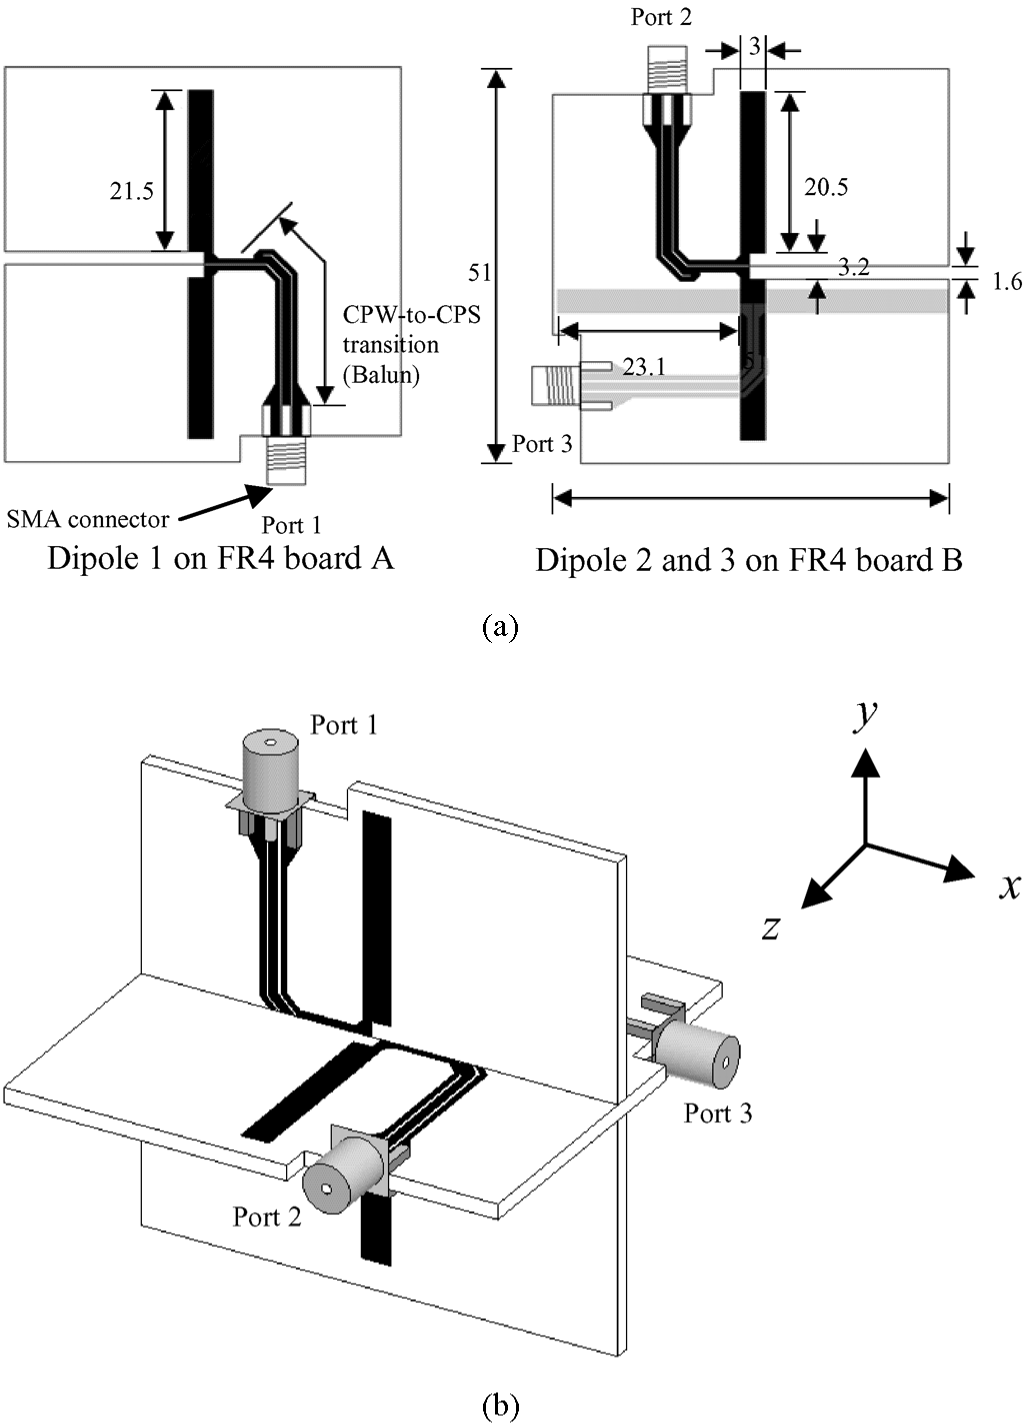
\includegraphics[width=.95\columnwidth]{figure52}
\caption{MPoA di tre dipoli stampati progettato per sistemi MIMO.}
\label{fig:52}
\end{figure}

\subsubsection{Diversità  di pattern}

\par Le antenne vengono progettate in modo da generare pattern ortogonali. Tipicamente viene realizzato mediante MMA Fig. \ref{fig:22}-\ref{fig:23} o con reti di {beamforming} quali la matrice di Butler Fig. \ref{fig:24}-\ref{fig:25}.
\begin{figure}[!h]
\centering
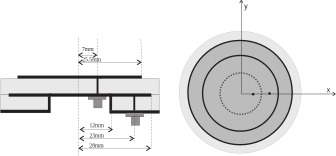
\includegraphics[width=.9\columnwidth]{figure22}
\caption{MMA realizzato in struttura planare con la sovrapposizione di patch circolari \cite{Herscovici}.}
\label{fig:22}
\end{figure}

\begin{figure}[!h]
\centering
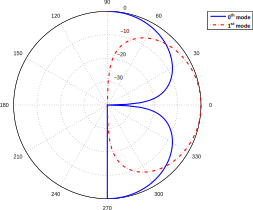
\includegraphics[width=.65\columnwidth]{figure23}
\caption{Pattern relativo all'MMA di Fig. \ref{fig:22}.}
\label{fig:23}
\end{figure}

\begin{figure}[!h]
\centering
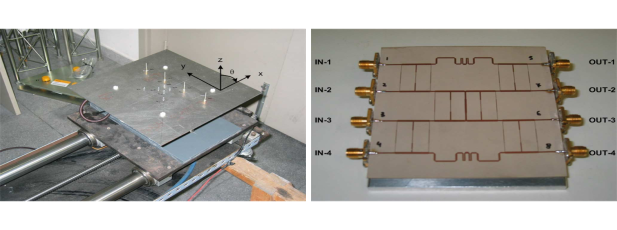
\includegraphics[width=.9\columnwidth]{figure24}
\caption{Array di 4 monopoli (sinistra) e matrice di Butler usata per il \textit{beamforming} (destra) \cite{Grau2006}.}
\label{fig:24}
\end{figure}


\begin{figure}[!h]
\centering
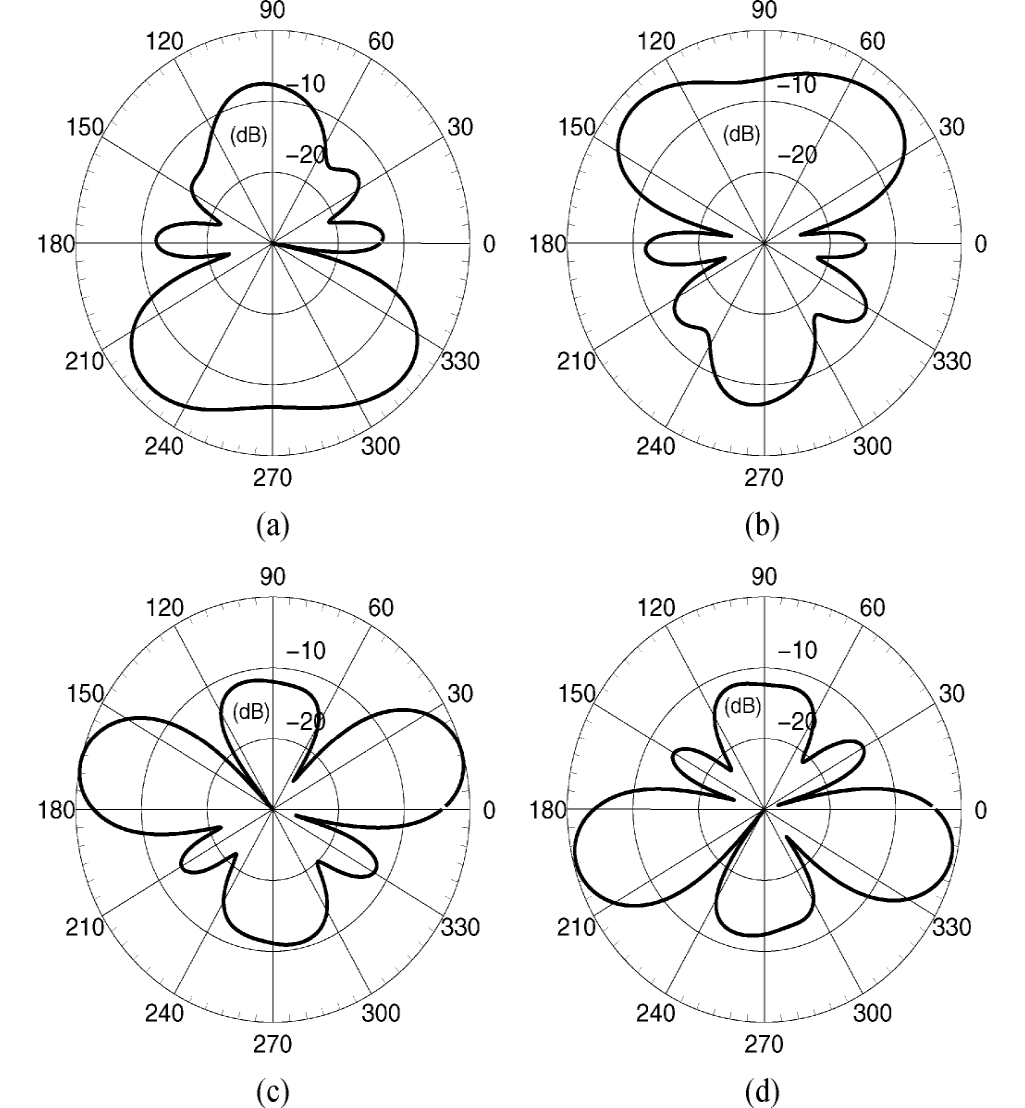
\includegraphics[width=.9\columnwidth]{figure25}
\caption{Pattern relativo alla struttura radiante di Fig. \ref{fig:24}, al variare della porta di eccitazione della matrice di Butler.}
\label{fig:25}
\end{figure}

\subsection{Reti di decorrelazione}

\begin{figure}[!h]
\centering
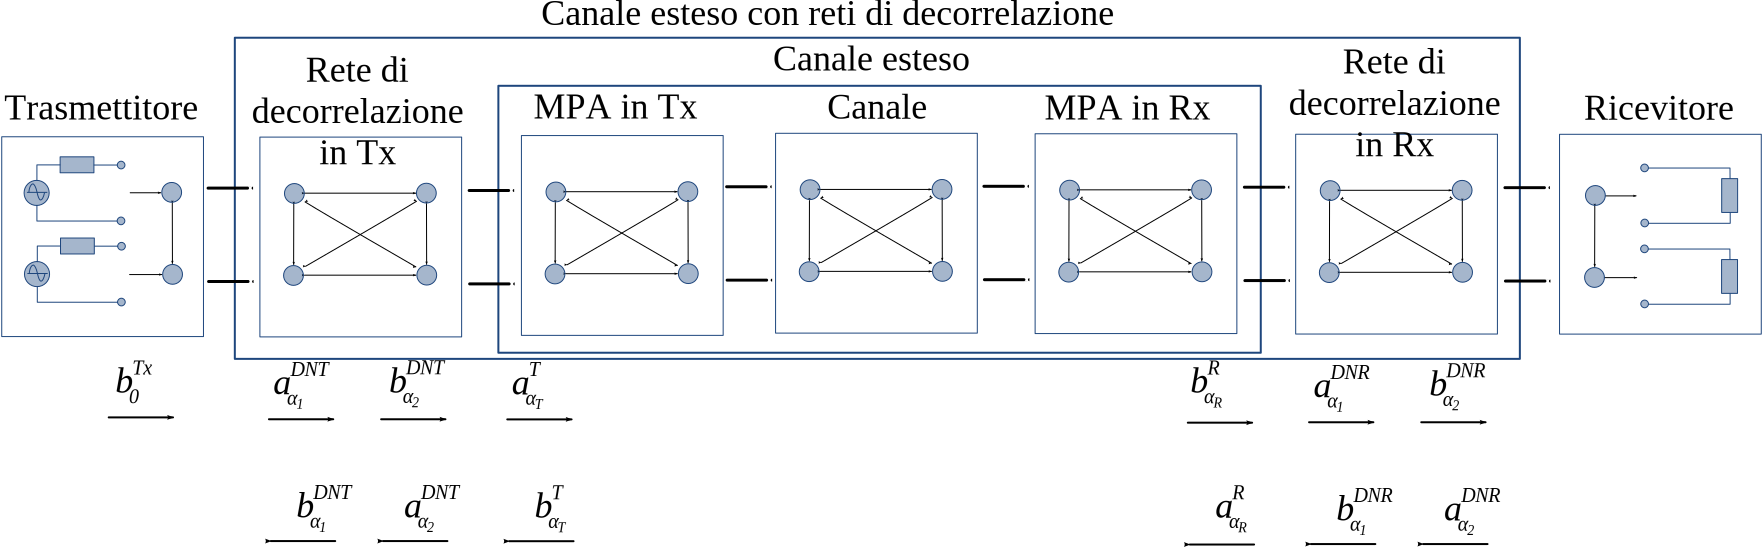
\includegraphics[width=\columnwidth]{figure26}
\caption{Modello di sistema con reti di decorrelazione.}
\label{fig:26}
\end{figure}


\par Le reti di decorrelazione (Fig. \ref{fig:26}) hanno lo scopo di compensare gli effetti dei mutui accoppiamenti mediante combinazioni lineari dei segnali ricevuti, sfruttando le simmetrie strutturali degli MPA. Il progetto si conduce anche qui separando Tx da Rx nello schema a blocchi. L'adattamento prediletto per la sintesi di DN è quello coniugato multiporta, ossia che tutte le porte siano adattate quando tutte le porte del sistema radiante sono eccitate. Si noti che comunque, in generale, l'impiego di DNs è tale da ridurre la banda operativa del sistema MIMO, essendo la circuiteria a banda relativamente stretta rispetto a quella delle antenne.

\section{Esempio di progetto di antenne per MIMO}

\par Si vogliono migliorare le prestazioni di un router wireless SISO (Fig. \ref{fig:27}) integrandovi funzionalità MIMO. Le dimensioni del router sono fisse ed è possibile aggiungere fino a due antenne. Assumendo il canale NLOS ideale, la correlazione tra le antenne si può valutare semplicemente dai coefficienti di mutuo accoppiamento. Si procede quindi con la loro simulazione mediante un CAD full-wave (HFSS\texttrademark), realizzandovi un modello (Fig. \ref{fig:28}) approssimativo ma elettromagneticamente analogo al router reale.

\begin{figure}[!ht]
\centering
\includegraphics[width=.5\columnwidth]{figure27}
\caption{Router SISO da migliorare, aggiungendovi funzionalità MIMO.}
\label{fig:27}
\end{figure}
\begin{figure}[!ht]
\centering
\includegraphics[width=.9\columnwidth]{figure28}
\caption{Modello equivalente HFSS.}
\label{fig:28}
\end{figure}

\par Avendo eseguito la simulazione, il coefficiente di scattering ottenuto a 2.43 GHz vale ${\bf{S}}_{{\alpha _T}{\alpha _T}}^{T} = 0.015 + j0.190$. Il coefficiente di correlazione d'antenna è dato da $${\bf{X}}_H^T = \frac{1}{{8\pi }}\left( {{\bf{I}} - {\bf{S}}_{{\alpha _T}{\alpha _T}}^T {{\left( {{\bf{S}}_{{\alpha _T}{\alpha _T}}^T} \right)}^\dagger}} \right),$$ e ${\bf{R}}_H^T = 1$ essendo il sistema a singola antenna. L'efficienza di adattamento, ossia il rapporto tra la potenza accettata dall'antenna e quella erogata dal generatore, è di 96 \%.                                             

\begin{figure}[!ht]
\centering
\includegraphics[width=.8\columnwidth]{figure29}
\caption{$S_{11}$ del sistema SISO al variare della frequenza.}
\label{fig:29}
\end{figure}

Assumendo un SNR di 10 dB, si calcola la distribuzione cumulativa della capacità di sistema (Fig. \ref{fig:30}).
\begin{figure}[!ht]
\centering
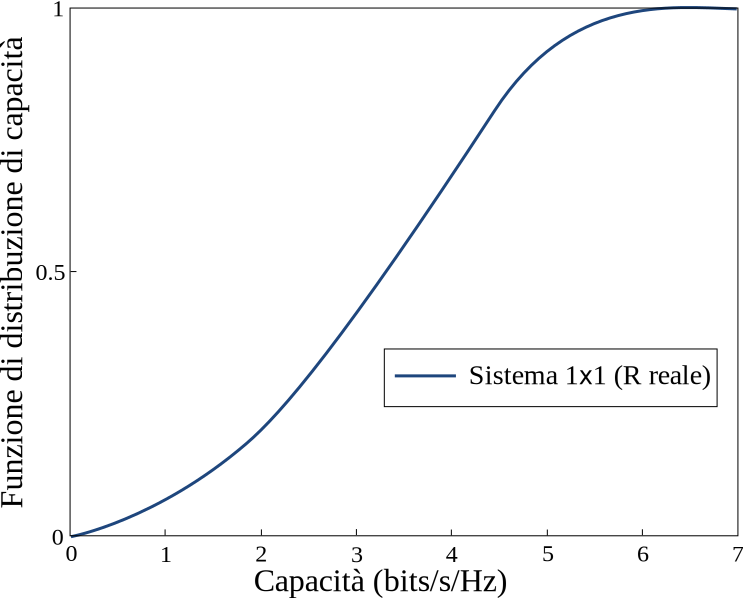
\includegraphics[width=.8\columnwidth]{figure30}
\caption{Distribuzione cumulativa della capacità di comunicazione del sistema SISO.}
\label{fig:30}
\end{figure}

\begin{figure}[!ht]
\centering
\includegraphics[width=\columnwidth]{figure31}
\caption{Router MIMO a due antenne.}
\label{fig:31}
\end{figure}

\par Si procede aggiungendo un'antenna al sistema, realizzando un router con due antenne spaziate di 40 cm ($\approx 3,3 \lambda$, Fig. \ref{fig:31}). Si ottiene dalla simulazione la seguente matrice di scattering:
\[ \scriptstyle { {\bf{S}}_{{\alpha _T}{\alpha _T}}^T = \left( {\begin{array}{*{20}{c}} \scriptstyle
{0.055 - j0.211}&\scriptstyle{ - 0.123 - j0.133}\\
\scriptstyle{ - 0.123 - j0.133}&\scriptstyle{0.055 - j0.253}
\end{array}} \right) } \] In Fig. \ref{fig:32}-\ref{fig:33} si hanno al variare della frequenza, rispettivamente, i coefficienti di riflessione $S_{11}$ e $S_{22}$ alle porte di eccitazione delle antenne e il coefficiente di accoppiamento $S_{21}$ tra le antenne. Si noti che $S_{12}=S_{21}$ per la reciprocità della struttura (i materiali usati nel modello HFSS sono privi di perdite).
L'efficienza di adattamento associata alla struttura radiante complessiva è di 86 \%.
\begin{figure}[!ht]
\centering
\includegraphics[width=.9\columnwidth]{figure32}
\caption{$S_{11}$ e $S_{22}$ simulati per il modello MIMO a due antenne.}
\label{fig:32}
\end{figure}
\begin{figure}[!ht]
\centering
\includegraphics[width=0.9\columnwidth]{figure33}
\caption{Coefficiente $S_{21}$ di mutuo accoppiamento nel sistema a due antenne.}
\label{fig:33}
\end{figure} La matrice di correlazione che avremmo nel caso ideale è un matrice unitaria $2 \times 2$: ${\bf{R}}_H^T = {\bf{I}}$. Siccome la matrice di scattering dell'MPA non è nulla, si ottiene una matrice di correlazione reale non unitaria pari a:
\[ \scriptstyle {\bf{R}}_H^T = \left( {\begin{array}{*{20}{c}}
\scriptstyle 1&\scriptstyle{ - 0.0530 - j0.0057}\\
\scriptstyle{ - 0.0530 - j0.0057}& \scriptstyle 1
\end{array}} \right)\]
In Fig. \ref{fig:34} vi è illustrata la distribuzione cumulativa di capacità relativa al sistema a due antenne nel caso di correlazione ideale e reale, avendo assunto come SNR in ricezione il valore di 10 dB.

\begin{figure}[!ht]
\centering
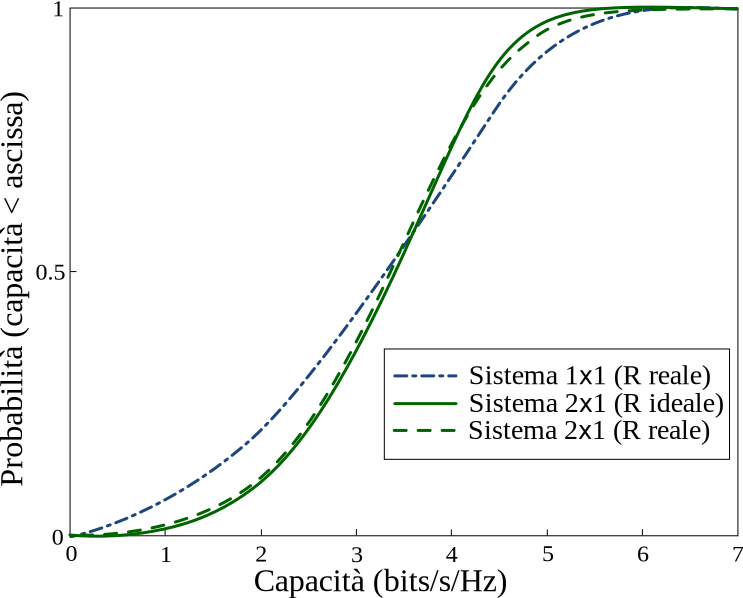
\includegraphics[width=.8\columnwidth]{figure34}
\caption{Distribuzione cumulativa di capacità per il sistema a due antenne.}
\label{fig:34}
\end{figure}

\par Aggiungendo infine un'altra antenna al router, si giunge alla condizione illustrata in Fig. \ref{fig:40}.
\begin{figure}[!ht]
\centering
\includegraphics[width=.9\columnwidth]{figure40}
\caption{Router MIMO a tre antenne.}
\label{fig:40}
\end{figure} 
I coefficienti di riflessione e quelli di accoppiamento al variare della frequenza sono illustrati in Fig. \ref{fig:35}-\ref{fig:36}.
\begin{figure}[!ht]
\centering
\includegraphics[width=.8\columnwidth]{figure35}
\caption{Modulo dei coefficienti di riflessione del sistema a tre antenne.}
\label{fig:35}
\end{figure}
\begin{figure}[!ht]
\centering
\includegraphics[width=.8\columnwidth]{figure36}
\caption{Modulo dei coefficienti di accoppiamento del sistema a tre antenne.}
\label{fig:36}
\end{figure}
Alla frequenza di 2.43 GHz, si ha la seguente matrice di scattering:
\[\scriptstyle {{\bf{S}}_{{\alpha _T}{\alpha _T}}^T = \left( {\begin{array}{*{20}{c}}
\scriptstyle{0.033 - j0.033}&\scriptstyle{0.105 - j0.450}&\scriptstyle{ - 0.122 + j0.015}\\
\scriptstyle{0.105 - j0.450}&\scriptstyle{0.167 + j0.400}&\scriptstyle{0.086 - j0.468}\\
\scriptstyle{0.105 - j0.450}&\scriptstyle{0.105 - j0.450}&\scriptstyle{0.059 - j0.061}
\end{array}} \right) }\]
e un'efficienza di adattamento complessiva di 74 \%. La matrice di correlazione si discosta dal caso ideale (matrice unitaria) in modo più significativo rispetto al sistema a due antenne:
\[\scriptstyle{ {\bf{R}}_H^T = \left( {\begin{array}{*{20}{c}}
\scriptstyle 1&\scriptstyle{0.3022 + j0.3020}&\scriptstyle{ - 0.2747 - j0.0293}\\
\scriptstyle{0.3022 + j0.3020}&\scriptstyle 1&\scriptstyle{0.4083 - j0.2516}\\
\scriptstyle{ - 0.2747 - j0.0293}&\scriptstyle{0.4083 - j0.2516}&\scriptstyle 1
\end{array}} \right) }\] In effetti, non si ha una variazione significativa nella distribuzione cumulativa di capacità (Fig. \ref{fig:37}).

\begin{figure}[!ht]
\centering
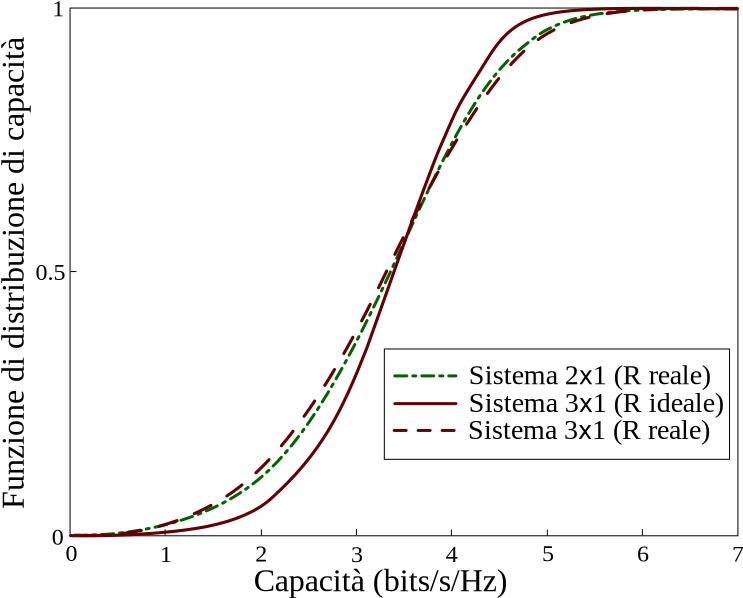
\includegraphics[width=0.8\columnwidth]{figure37}
\caption{Distribuzione cumulativa di capacità dei sistemi a due e tre antenne.}
\label{fig:37}
\end{figure}
La capacità media (ergodica) dei tre sistemi, ossia la capacità riportata dalla distribuzione cumulativa raggiunta una probabilità di 50 \%, viene riportata nella Tab. \ref{tab:sistemi}. Si noti come il sistema a tre antenne presenti prestazioni peggiori rispetto a quello con due antenne. Questo è riconducibile alla perdita di potenza utile alla comunicazione, in gran parte dovuta ai forti accoppiamenti mutui tra le antenne che si ritrovano ulteriormente ravvicinate (20 cm rispetto ai 40 cm del sistema a due antenne).
\begin{table}[h!]
\begin{center}
\begin{tabular}{|c|c|}
\hline
Sistema & Capacità [bits/s/Hz] \\ \hline \hline
$1 \times 1$ & 3.1848 \\ \hline
$2 \times 1$ & 3.3045 \\ \hline
$3 \times 1$ & 3.2869 \\ \hline
\end{tabular}
\end{center}
\caption{Capacità media dei sistemi MIMO analizzati.}
\label{tab:sistemi}
\end{table}

%\begin{figure}[!ht]
%\centering
%\includegraphics[width=\columnwidth]{figure38}
%\caption{Distribuzione cumulativa di capacità dei sistemi a 2 e tre antenne.}
%\label{fig:38}
%\end{figure}

\par Si analizzi il comportamento del sistema MIMO illustrato in Fig. \ref{fig:39}. Come si comporta nei confronti dei mutui accoppiamenti rispetto ai precedenti sistemi? Possiamo aspettarci una capacità maggiore?
\begin{figure}[!ht]
\centering
\includegraphics[width=.8\columnwidth]{figure39}
\caption{Router MIMO a due antenne con polarizzazioni ortogonali.}
\label{fig:39}
\end{figure}

\section{Conclusione}

\par Introducendo la ``diversità spaziale'', il progetto di antenne per sistemi MIMO richiede in generale la conoscenza delle caratteristiche di propagazione del canale di comunicazione wireless. La presenza di propagazione non diretta tra trasmettitore e ricevitore ma per cammini multipli consente di migliorare le prestazioni di comunicazione, purché non vi sia forte correlazione tra i vari cammini.

 I sistemi radianti in trasmissione e ricezione, eventuali reti di decorrelazione ed il canale possono essere modellati mediante matrici di scattering. La divisione in sottoblocchi del sistema consente di ottimizzare, a seconda delle necessità, ciascuna parte del sistema per un aumento complessivo delle prestazioni. 
 
Nell'ipotesi di propagazione ricca di scattering, è possibile semplificare il progetto del sistema MIMO limitandosi ad ottimizzare l'adattamento delle antenne (adattamento coniugato multiporta) e minimizzando opportunamente gli accoppiamenti. 

Vi sono tre tipologie d'antenne che consentono di implementare la diversità spaziale, ossia gli array di antenne identiche opportunamente distanziate, quelli di antenne polarizzate diversamente e i sistemi radianti che sintetizzano pattern ortogonali (che coprono angoli solidi distinti) a seconda della porta di eccitazione scelta.

% The very first letter is a 2 line initial drop letter followed
% by the rest of the first word in caps.
% 
% form to use if the first word consists of a single letter:
% \IEEEPARstart{A}{demo} file is ....
% 
% form to use if you need the single drop letter followed by
% normal text (unknown if ever used by IEEE):
% \IEEEPARstart{A}{}demo file is ....
% 
% Some journals put the first two words in caps:
% \IEEEPARstart{T}{his demo} file is ....
% 
% Here we have the typical use of a "T" for an initial drop letter
% and "HIS" in caps to complete the first word.
%\IEEEPARstart{T}{his} demo file is intended to serve as a ``starter file''
%for IEEE journal papers produced under \LaTeX\ using
%IEEEtran.cls version 1.7 and later.
% You must have at least 2 lines in the paragraph with the drop letter
% (should never be an issue)
%I wish you the best of success.

%\hfill mds
% 
%\hfill January 11, 2007





%\%subsection{Subsection Heading Here}
%Subsection text here.

% needed in second column of first page if using \IEEEpubid
%\IEEEpubidadjcol

%\%subsubsection{Subsubsection Heading Here}
%Subsubsection text here.


% An example of a floating figure using the graphicx package.
% Note that \label must occur AFTER (or within) \caption.
% For figures, \caption should occur after the \includegraphics.
% Note that IEEEtran v1.7 and later has special internal code that
% is designed to preserve the operation of \label within \caption
% even when the captionsoff option is in effect. However, because
% of issues like this, it may be the safest practice to put all your
% \label just after \caption rather than within \caption{}.
%
% Reminder: the "draftcls" or "draftclsnofoot", not "draft", class
% option should be used if it is desired that the figures are to be
% displayed while in draft mode.
%
%\begin{figure}[!t]
%\centering
%\includegraphics[width=2.5in]{myfigure}
% where an .eps filename suffix will be assumed under latex, 
% and a .pdf suffix will be assumed for pdflatex; or what has been declared
% via \DeclareGraphicsExtensions.
%\caption{Simulation Results}
%\label{fig_sim}
%\end{figure}

% Note that IEEE typically puts floats only at the top, even when this
% results in a large percentage of a column being occupied by floats.


% An example of a double column floating figure using two subfigures.
% (The subfig.sty package must be loaded for this to work.)
% The subfigure \label commands are set within each subfloat command, the
% \label for the overall figure must come after \caption.
% \hfil must be used as a separator to get equal spacing.
% The subfigure.sty package works much the same way, except \subfigure is
% used instead of \subfloat.
%
%\begin{figure*}[!t]
%\centerline{\subfloat[Case I]\includegraphics[width=2.5in]{subfigcase1}%
%\label{fig_first_case}}
%\hfil
%\subfloat[Case II]{\includegraphics[width=2.5in]{subfigcase2}%
%\label{fig_second_case}}}
%\caption{Simulation results}
%\label{fig_sim}
%\end{figure*}
%
% Note that often IEEE papers with subfigures do not employ subfigure
% captions (using the optional argument to \subfloat), but instead will
% reference/describe all of them (a), (b), etc., within the main caption.


% An example of a floating table. Note that, for IEEE style tables, the 
% \caption command should come BEFORE the table. Table text will default to
% \footnotesize as IEEE normally uses this smaller font for tables.
% The \label must come after \caption as always.
%
%\begin{table}[!t]
%% increase table row spacing, adjust to taste
%\renewcommand{\arraystretch}{1.3}
% if using array.sty, it might be a good idea to tweak the value of
% \extrarowheight as needed to properly center the text within the cells
%\caption{An Example of a Table}
%\label{table_example}
%\centering
%% Some packages, such as MDW tools, offer better commands for making tables
%% than the plain LaTeX2e tabular which is used here.
%\begin{tabular}{|c||c|}
%\hline
%One & Two\\
%\hline
%Three & Four\\
%\hline
%\end{tabular}
%\end{table}


% Note that IEEE does not put floats in the very first column - or typically
% anywhere on the first page for that matter. Also, in-text middle ("here")
% positioning is not used. Most IEEE journals use top floats exclusively.
% Note that, LaTeX2e, unlike IEEE journals, places footnotes above bottom
% floats. This can be corrected via the \fnbelowfloat command of the
% stfloats package.



%\%section{Conclusion}

%The conclusion goes here.





% if have a single appendix:
%\appendix[Proof of the Zonklar Equations]
% or
%\appendix  % for no appendix heading
% do not use \section anymore after \appendix, only \section*
% is possibly needed

% use appendices with more than one appendix
% then use \section to start each appendix
% you must declare a \section before using any
% \subsection or using \label (\appendices by itself
% starts a section numbered zero.)
%


%\appendices
%\%section{Proof of the First Zonklar Equation}
%Appendix one text goes here.

% you can choose not to have a title for an appendix
% if you want by leaving the argument blank
%\%section{}
%Appendix two text goes here.


% use section* for acknowledgement
%\%section*{Acknowledgment}


%The authors would like to thank...


% Can use something like this to put references on a page
% by themselves when using endfloat and the captionsoff option.
\ifCLASSOPTIONcaptionsoff
  \newpage
\fi



% trigger a \newpage just before the given reference
% number - used to balance the columns on the last page
% adjust value as needed - may need to be readjusted if
% the document is modified later
%\IEEEtriggeratref{8}
% The "triggered" command can be changed if desired:
%\IEEEtriggercmd{\enlargethispage{-5in}}

% references section

% can use a bibliography generated by BibTeX as a .bbl file
% BibTeX documentation can be easily obtained at:
% http://www.ctan.org/tex-archive/biblio/bibtex/contrib/doc/
% The IEEEtran BibTeX style support page is at:
% http://www.michaelshell.org/tex/ieeetran/bibtex/
%\bibliographystyle{IEEEtran}
% argument is your BibTeX string definitions and bibliography database(s)
%\bibliography{IEEEabrv,../bib/paper}
%
% <OR> manually copy in the resultant .bbl file
% set second argument of \begin to the number of references
% (used to reserve space for the reference number labels box)
%\begin{thebibliography}{1}
%
%\bibitem{IEEEhowto:kopka}
%H.~Kopka and P.~W. Daly, \emph{A Guide to \LaTeX}, 3rd~ed.\hskip 1em plus
%  0.5em minus 0.4em\relax Harlow, England: Addison-Wesley, 1999.
%
%\end{thebibliography}

\bibliographystyle{IEEEtran}	% (uses file "plain.bst")
\bibliography{MIMO}	

% biography section
% 
% If you have an EPS/PDF photo (graphicx package needed) extra braces are
% needed around the contents of the optional argument to biography to prevent
% the LaTeX parser from getting confused when it sees the complicated
% \includegraphics command within an optional argument. (You could create
% your own custom macro containing the \includegraphics command to make things
% simpler here.)
%\begin{biography}[{\includegraphics[width=1in,height=1.25in,clip,keepaspectratio]{mshell}}]{Michael Shell}
% or if you just want to reserve a space for a photo:

%\begin{IEEEbiography}{Michael Shell}
%Biography text here.
%\end{IEEEbiography}

% if you will not have a photo at all:
%\begin{IEEEbiographynophoto}{John Doe}
%Biography text here.
%\end{IEEEbiographynophoto}

% insert where needed to balance the two columns on the last page with
% biographies
%\newpage

%\begin{IEEEbiographynophoto}{Jane Doe}
%Biography text here.
%\end{IEEEbiographynophoto}

% You can push biographies down or up by placing
% a \vfill before or after them. The appropriate
% use of \vfill depends on what kind of text is
% on the last page and whether or not the columns
% are being equalized.

%\vfill

% Can be used to pull up biographies so that the bottom of the last one
% is flush with the other column.
%\enlargethispage{-5in}



% that's all folks
\end{document}


